\documentclass[12pt,a4paper,notitlepage]{article}
\usepackage[utf8x]{inputenc}
\usepackage[T1]{fontenc}
\usepackage{ucs}
\usepackage[english]{babel}
\usepackage{amsmath}
\numberwithin{equation}{section}
\usepackage{longtable}
\usepackage{supertabular}
\usepackage{pdfpages}
\usepackage{threeparttablex}
\DeclareMathOperator*{\argmax}{arg\,max}
\DeclareMathOperator*{\argmin}{arg\,min}
\usepackage{amsfonts}
\usepackage[shortlabels]{enumitem}
\usepackage{amssymb}
\usepackage{graphicx}
\usepackage{float}
\usepackage{url}
\usepackage{multirow}
\usepackage{makecell}
\usepackage[left=2.8cm, right=2.8cm, top=2.5cm, bottom=2.5cm]{geometry}

\begin{document}
\thispagestyle{empty}

\begin{figure}[H]
    \centering
    
\includegraphics[width=0.3\textwidth]{LogoMLU.pdf}
\end{figure}

\begin{center}
    Martin Luther University Halle-Wittenberg \\
    Chair of Economics, especially Macroeconomics \\
    Professor Dr Oliver Holtemöller
\end{center}

\vspace*{3.5cm}

\begin{center}
    {\Huge\bf Advanced Macroeconomics} \\[0.5cm]
    {\Large\bf Exam Winter 2024/2025} \\[0.5cm]
    {\large\bf Problem Set \#n } \\[0.5cm]
\end{center}

\vspace*{3.5cm}

\noindent

	\vspace*{3.5cm}
	************************************** \\	
	************ Student Data ************ \\
	Name: Tahereh Parnian\\ tahereh.parnian@student.uni-halle.de\\StudentID- 222221306\\problem set ID \#n
 \\
	
	**************************************
	
	\vspace*{1cm}
	
	********* 05 August 2025 ********
	


\newpage


\pagenumbering{arabic}
\tableofcontents
\listoffigures 
\listoftables

\newpage
\thispagestyle{plain}
	
\section*{Overview of Code Files}
\begin{table}[h]
	\begin{center}
		\begin{tabular}{|c|c|c|}
			\hline
			\textbf{File Name} & \textbf{File Description} & \textbf{Reference Files} \\ \hline
			\makecell{\texttt{Data.R} }& \makecell{Loads and filters Eurostat raw data \\ Keeps only Czech Republic entries \\ Renames and exports cleaned dataset}& \makecell{\texttt Example\_4\_3.m} \\ \hline
			{\texttt{problemset11.m}}& \makecell{Solves Task 1.1: \\ Loads cleaned Czech consumption data \\ Plots time series for durables and non-durables \\ MATLAB/Octave compatible visual output } & 
            \makecell{\texttt Example\_4\_4.m}} \\ \hline
			\makecell{ \texttt{problemset13.m}} & \makecell{Solves Task 1.2: \\ Implements one-period consumption model \\ Calculates $c_1$, $c_2$ across preference weights \\ Plots consumption vs.\ $\omega$} 	& \makecell{\texttt Example\_4\_5.m} \\ \hline
            \makecell{\texttt{Data.pwt.R}} & 
\makecell{Loads PWT data \\ Filters India (IND) only \\ Exports GDP \& investment share} & 
\makecell{\texttt Example\_4\_3.m } \\ \hline

\makecell{\texttt{problemset21.m}} & 
\makecell{Solve Task 2.1:\\ Plot GDP and investment share \\ from PWT data with average line} & 
\makecell{\texttt Self-written,\\  empirical analysis } \\ \hline
\makecell{\texttt{ramsey\_ishare.mod}} & 
\makecell{define variables (endogenous and exogenous) \\
define parameters including \texttt{ishare} \\
set steady-state equations \\
solve model for different $\rho$
} & 
\texttt{ramsey\_ishare.mod} \\ \hline

\makecell{\texttt{problemset22.m}} & 
\makecell{Solves Task 2.2: \\
Extended Ramsey model \\
Write a for loop over $\rho$ \\
Compute steady-state I/Y and Y \\
Plot both as functions of $\rho$
} & 
\texttt{ramsey\_ishare.mod} \\ \hline

\makecell{\texttt{moncomp\_stoch\_h0\_0.mod}} & 
\makecell{Simulates stochastic NK model \\
without habit persistence ($h = 0$). \\
Computes IRFs to technology shocks.
} & 
\texttt{moncomp\_stoch.mod} \\ \hline 


\makecell{\texttt{moncomp\_stoch\_h0\_4.mod}} & 
\makecell{Simulates stochastic NK model \\
with moderate habit persistence ($h = 0.4$). \\
Computes IRFs to technology shocks.
} & 
\texttt{moncomp\_stoch.mod} \\ \hline 

  \texttt{moncomp\_stoch\_h0\_7.mod} & 
			\makecell{with high habit persistence ($h = 0.7$)} & 
			 \texttt{moncomp\_stoch.mod} \\ \hline

          \texttt{problemset32.m} & 
			\makecell{Simulate and plots IRF } & 
			 \texttt{moncomp\_stoch.mod} \\ \hline

           

            
        \end{tabular}  
		\caption{Table of code files. }
	\end{center}
\end{table}




\textbf{}
\newpage

\section*{Data File}
\begin{table}[h]
	\begin{center}
		\begin{tabular}{|c|c|c|}
			\hline
			\textbf{Data ID} & \textbf{Data Description} & \textbf{Data Source} \\ \hline
			
			\makecell{\texttt{estat\_namq\_10\_fcs\_} \\
			\texttt{filtered\_en.csv}} & 
			\makecell{Raw Eurostat data (Czech Republic) \\
			Includes food, non-durables \& services \\
			Seasonally adjusted, 2010 prices} & 
			Eurostat \\ \hline
			
			\texttt{cz\_clean\_consumption.csv} & 
			\makecell{Cleaned version of Eurostat data \\
			Only Czech Republic, reshaped wide \\
			Missing values removed, variables renamed} & 
			Eurostat \\ \hline
			
			\texttt{pwt1001.xlsx} & 
            \makecell{Penn World Table data \\
            Cross-country macroeconomic indicators \\ Used for growth and comparison analysis} & 
            \makecell{Penn World Table \\ (10.01)} \\ \hline

			\texttt{pwt1001\_IND.csv} & 
            \makecell{PWT data for India only \\
             Includes real GDP and investment share \\
            Used in Task 2.1 to analyze long-run growth} & 
            \makecell{Penn World Table \\ (10.01)} \\ \hline

			
			
			
		\end{tabular}
		\caption{Table of data.}
	\end{center}
\end{table}



\newpage

\section {Part I }

 \subsection{Task 1: Household Consumption Data from Eurostat} 
  \subsubsection {   Access Empirical Data}

For Task 1, Household Consumption, I downloaded quarterly data on household consumption expenditures from the \texttt{Eurostat}\footnote{\url{https://ec.europa.eu/eurostat/databrowser/view/namq_10_fcs/default/table?lang=en&category=na10.namq_10.namq_10_ma}} database, focusing on the Czech Republic as assigned by my digiMOPS code (EW48q7).


I accessed the Eurostat Data Browser and searched for the dataset \texttt{namq\_10\_fcs}. After selecting the dataset, I customized the download by applying the following filters:

\begin{itemize}
  \item \textbf{National accounts items:} \\
  P311\_S14 (Durable goods), P312N\_S14 (Non-durables and services)

  \item \textbf{Unit of measure:} \\
  CLV10\_MEUR (Chain-linked volumes, million euros)

  \item \textbf{Seasonal adjustment:} \\
  SCA (Seasonally and calendar adjusted)

  \item \textbf{Geographical area:} \\
  Czech Republic

  \item \textbf{Time period:} \\
  From 2010-Q1 to the most recent quarter

  \item \textbf{Frequency:} \\
  Quarterly
\end{itemize}

After applying the filters, I downloaded the file \texttt{estat\_namq\_10\_fcs\_filtered\_en.csv} from the Eurostat Data Browser. The dataset contains {quarterly household consumption expenditure data}. Following the project instructions, I initially intended to process the raw dataset in \texttt{R}\footnote{See \url{https://posit.co/downloads/}. } and prepared the cleaned version using the code provided in the file titled \texttt{Data.R}. 

From the downloaded file, I extracted the relevant information for the Czech Republic — my assigned country — and saved the resulting cleaned dataset as \\ \texttt{cz\_clean\_consumption.csv}.


This cleaned file contains separate time series for the consumption of durable goods (\texttt{P311\_S14}) and non-durables/services (\texttt{P312N\_S14}), structured in a format compatible with \texttt{MATLAB}\footnote{See \url{https://matlab.mathworks.com}.}. I then refined the dataset in MATLAB by renaming variables, standardizing date formats, and converting numeric values where necessary.

This two-step process — downloading the comprehensive dataset and extracting the relevant country-level data — ensured compliance with the project's formal requirements while maintaining a transparent and reproducible workflow.

Both series were visualized to assess their behavior over time. The consumption of non-durables and services is consistently higher and more stable, whereas the durable goods component is smaller and exhibits greater volatility, especially during economic shocks such as COVID-19. A noticeable decline in both series occurs around 2020, followed by a gradual recovery.

The corresponding graph is presented later in this section.

\subsubsection{   file: Problemset11.m}
For solving this task with \texttt{Octave}\footnote{See \url {https://octave.org/index}.} or \texttt{Matlab}\footnote{See \url{https://de.mathworks.com/products/matlab.html}.} \ The  lecture 4 file and \texttt{ Example\_4\_4.m} is used to adjusted in steps as follows: 

\begin{itemize}
    \item The code begins by specifying the data source, author, and MATLAB version. It ensures compatibility with both MATLAB and Octave environments. A colorblind-friendly palette is defined for accessible visualizations. Then, it loads cleaned household consumption data from a CSV file and plots durable and non-durable goods over time.

    \item Initialize Environment Closes all open figures and sets up a figure counter. It checks whether the code is running in MATLAB or Octave and loads necessary packages if in Octave.
    \item Color Setup Defines a colorblind-friendly palette to ensure that the plots are accessible and visually distinct.
    \item Load-Cleaned Data Reads in the {cz\_clean\_consumption.csv} file, which contains Czech household consumption data for: 
	   \begin{itemize}
    \item[1.] \texttt{P311\_S14\_food\_bev}: Durable goods
    \item[2.] \texttt{P312N\_S14\_non\_durable\_excl\_food}: Non-durables \& services
\end{itemize}

    
	\item Format Time Series Converts the time column from "2010-Q1" format to a proper datetime object in MATLAB, creating a time axis for plotting. 
    \item Extract and Assign Variables Assigns the durable and non-durable consumption series to separate variables for clarity:
    \item Plot both series over time using distinguishable colors:
    \begin{itemize}
		\item[1.] Blue for durable goods
		\item[2.] Orange for non-durables and services
        
        Adds grid, legend, title, and axis labels for a clean presentation.
	    \end{itemize}
	\item Save the Plot	 as a .png file.
	\end{itemize}
    
\begin{figure} [H]
	\centering
	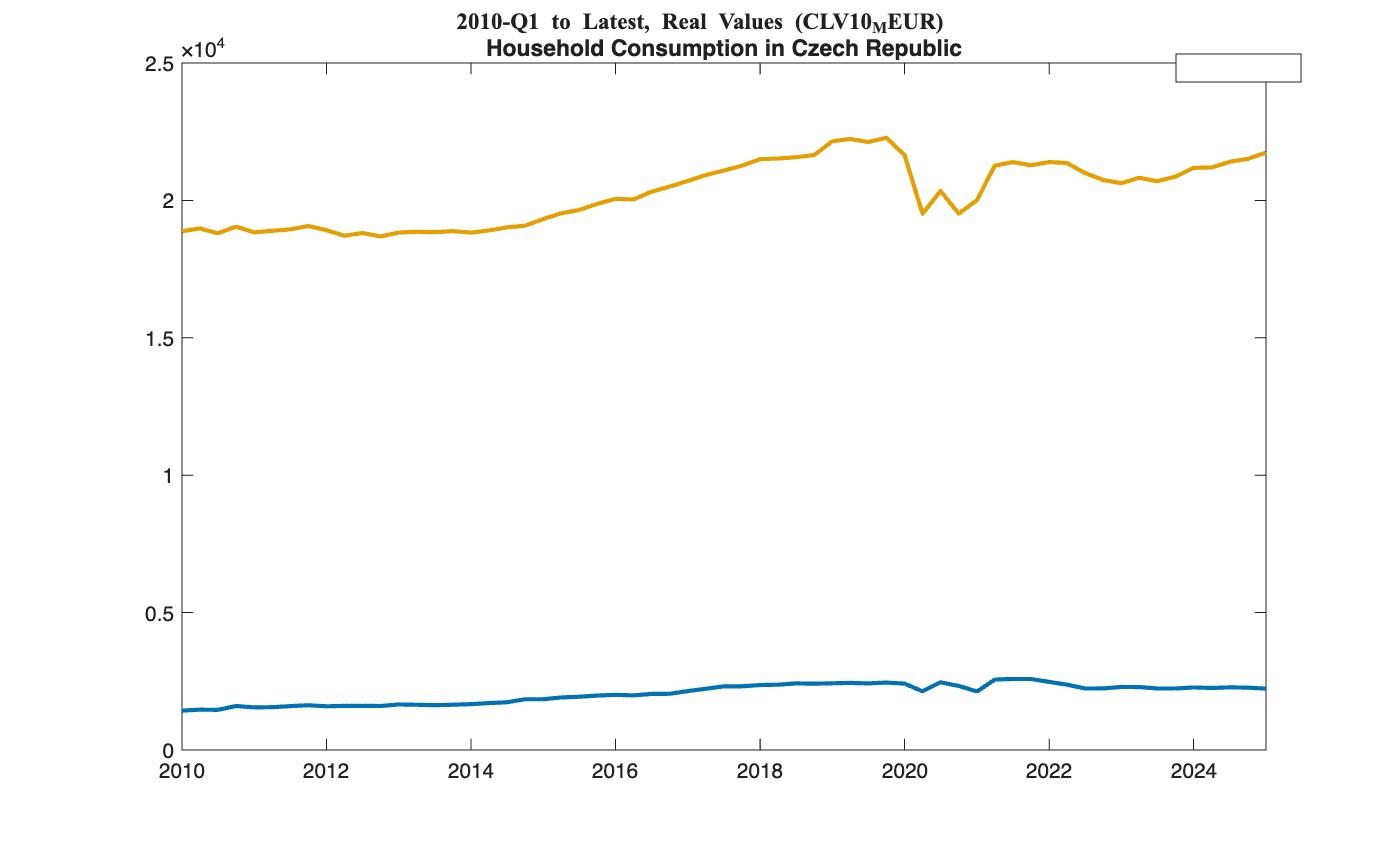
\includegraphics[width = 1 \textwidth]{HH Consumption_Cz.png}
	\label{fig:locally}
	\caption{Household Consumption Czech Republic.}
\end{figure}


The plot shown in Figure 1 and produced by code file \texttt{problemset11.m } reveals that Czech households consistently spend more on non-durable goods and services than on durable goods. Non-durable spending shows a steady upward trend, with a noticeable dip around 2020 due to the COVID-19 pandemic, followed by gradual recovery. Durable goods, on the other hand, exhibit more volatility and a smaller overall share of household consumption. Their fluctuations suggest sensitivity to economic uncertainty and changes in household income or interest rates.

\newpage


\subsection{Task 2: One-Period Model with Adjusted Utility}

We are given the utility function:
\[
u(c_1, c_2) = ({1-\omega}) \ln c_1 + \omega \ln c_2
\]

with:
\begin{itemize}
    \item $c_1$: consumption of good 1 (price normalized to 1),
    \item $c_2$: consumption of good 2 (price = $p$),
    \item $\omega \in (0,1)$: preference weight,
    \item Budget constraint: $c_1 + p c_2 = I$ with $I = w + r$.
\end{itemize}

\subsubsection{   Analytical Derivation of Optimal $c_1$ and $c_2$}

The household maximizes:
\[
\max_{c_1, c_2} \ ({1-\omega}) \ln c_1 + \omega \ln c_2 \quad \text
\]
\[
\text{subject to:} \quad c_1 + p \cdot c_2 = I, \quad \text{where } I = w + r
\]
\noindent \textbf{Lagrangian:}
\[
\mathcal{L} = ({1-\omega})\ln c_1 + \omega \ln c_2 + \lambda (I - c_1 - p c_2)
\]

\noindent \textbf{First-order conditions (FOCs):}
\[
\frac{\partial \mathcal{L}}{\partial c_1} = \frac{1-\omega}{c_1} - \lambda = 0
\quad \Rightarrow \quad \lambda = \frac{1-\omega}{c_1}
\]
\[
\frac{\partial \mathcal{L}}{\partial c_2} = \frac{\omega}{c_2} - \lambda p = 0
\quad \Rightarrow \quad \lambda = \frac{\omega}{p c_2}
\]

\noindent \textbf{Equating both expressions for $\lambda$:}
\[
\frac{1-\omega}{c_1} = \frac{\omega}{p c_2}
\quad \Rightarrow \quad c_2 = \frac{\omega}{(1-\omega)p} \cdot c_1
\]

\noindent \textbf{Substitute into budget constraint:}
\[
c_1 + p c_2 = I \Rightarrow c_1 + \frac{\omega}{1-\omega} c_1 = I
\Rightarrow c_1 \left(1 + \frac{\omega}{1-\omega}\right) = I
\Rightarrow c_1 = (1 - \omega) I
\]

\noindent \textbf{Then:}
\[
c_2 = \frac{\omega}{p} I
\]

\noindent \textbf{Conclusion:} These are the optimal consumption levels:
\[
c_1 = ({1-\omega})(w + r), \quad c_2 = \frac{\omega}{p}(w + r)
\]

\subsubsection{   Solve for Equilibrium Values  }

Given: $r = 0.2$, $w = 0.7$, $p = 1$, $\omega = 0.5$, hence $I = w + r = 0.9$.

\[
c_1 = (1−0.5)(0.9) = 0.45, \quad
c_2 = \frac{0.5}{1} \cdot 0.9 = 0.45
\]

\noindent \textbf{Result:} Both goods are consumed equally:
\[
c_1 = c_2 = 0.45
\]


\subsubsection{   Simulating and Plotting: \texttt{Problemset13.m}}

The purpose of \texttt{Problemset13.m} is to simulate how optimal consumption levels \( c_1 \) and \( c_2 \) change as the preference parameter \( \omega \) varies between 0.01 and 0.99. 

\begin{itemize}
    \item To do this we defines income $I = w + r$ and normalize the price $p = 1$.
    \item we calculates $c_1 = (1 - \omega) \cdot I$ and $c_2 = \omega \cdot I / p$ for a range of $\omega$ in this way we have:
\[
c_1(\omega) = (1 - \omega)(w + r), \quad
c_2(\omega) = \frac{\omega}{p}(w + r)
\]



\begin{figure} [H]
	\centering
	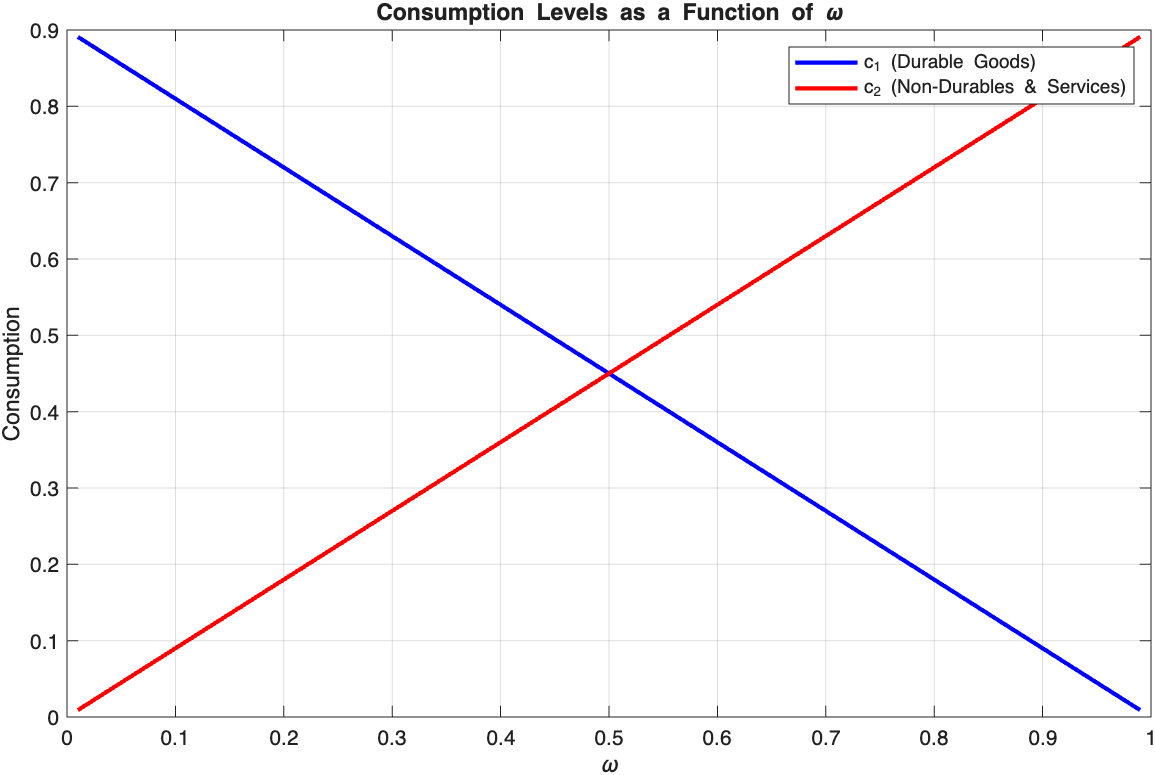
\includegraphics[width = 1 \textwidth]{Consumption Level.png}
	\label{fig:locally}
	\caption{Consumption Level as a Function of\ $\omega$.}
\end{figure}

The plot shown in \textbf{Figure 2}, produced using the file \texttt{problemset13.m}, illustrates how optimal consumption levels of two goods change as the preference parameter \( \omega \) varies between 0.01 and 0.99. This simulation is based on the theoretical utility function introduced in {Lecture 4}, where \( \omega \) represents the relative weight households place on non-durables and services in their utility.

As \( \omega \) increases:
\begin{itemize}
  \item \( c_1 \) (Durable goods) steadily declines — reflecting that households prioritize them less.
  \item \( c_2 \) (Non-durables \& services) rises — more of the budget is shifted toward this category.
\end{itemize}

At \( \omega = 0.5 \), consumption of both goods is equal: \( c_1 = c_2 = 0.45 \). This behavior is consistent with the theoretical relationship between utility weights and consumption allocation, as introduced in Lecture 4.

Importantly, the total budget \( I \) remains constant throughout the simulation. What changes is not income or price, but preferences. The simulation confirms the intuition that even when income and prices are fixed, varying the preference parameter \( \omega \) can significantly reshape the consumption bundle. It highlights that household consumption patterns are highly sensitive to shifts in preferences — what people want shapes how they spend.

\newpage
\section {Part II }

\subsection{Task 1: Growth and Investment – India (Penn World Tables)}
\subsubsection{   Access and Prepare Country-Level Data}

For Task 1, I used data from the \texttt{Penn World Table data}\footnote{See \url {\url{https://www.rug.nl/ggdc/productivity/pwt} \\}.}, which provides internationally comparable macroeconomic indicators. I began with the Excel file \texttt{pwt1001.xlsx}\footnote{Available at: \url{https://www.rug.nl/ggdc/productivity/pwt/}} containing data for over 180 countries.

To extract data specifically for India — my assigned country — I wrote an R script titled \texttt{Data\_PWT.R}. This script performs the following steps:

\begin{itemize}
  \item Loads the full Excel dataset using the \texttt{readxl} package.
  \item Filters the data for India using the country code \texttt{IND}.
  \item Selects key variables: \texttt{year}, \texttt{rgdpe} (real GDP), and \texttt{csh\_i} (investment share).
  \item Saves the cleaned, country-specific data as a CSV file named \texttt{pwt1001\_IND.csv}.
\end{itemize}

This dataset is formatted for direct use in \texttt{MATLAB}, enabling the analysis and visualization of long-run growth trends and investment shares. The workflow follows the structure introduced in \texttt{Example 4.3} of the lecture code files and ensures clarity, traceability, and compliance with the project’s documentation standards.


\subsubsection{   File: \texttt{Problemset21.m}}

To answer this task using \texttt{MATLAB}\footnote{See \url{https://www.mathworks.com/products/matlab.html}}, I created a script that reads in country-level data for India from the Penn World Table dataset and visualizes key macroeconomic indicators. The process follows the methodology seen in \texttt{Example\_4\_3.m}, with adjustments specific to the Indian context.


\begin{itemize}
    \item \textbf{Overview of Data} \\
    The script uses data from the Penn World Tables (version 10.01), focusing on India (\texttt{IND}) over the period from 1950 to the most recent available year. Two main variables are used:
    \begin{itemize}
        \item \texttt{rgdpe} – Expenditure-side real GDP at constant 2017 prices
        \item \texttt{csh\_i} – Share of gross capital formation in GDP (investment share)
    \end{itemize}

    \item \textbf{Load Cleaned Data} \\
    The script begins by loading the previously cleaned CSV file \texttt{pwt1001\_IND.csv}, which includes annual data for the variables listed above.

    \item \textbf{Extract Variables} \\
    It assigns the columns \texttt{year}, \texttt{rgdpe}, and \texttt{csh\_i} to corresponding variables in MATLAB.

    \item \textbf{Scale Investment Share for Plotting} \\
    Since the real GDP and investment share have different magnitudes, the investment share is scaled using a factor based on their respective maxima to allow for visual comparison on the same plot.

    \item \textbf{Compute and Plot Average Investment Share} \\
    The average investment share is computed (ignoring missing values) and drawn as a horizontal dashed line across the time series, representing its long-run mean.

    \item \textbf{Plot Time Series} \\
    The time series is visualized using two y-axes:
    \begin{itemize}
        \item \textcolor{blue}{Real GDP (left y-axis)} – shown in blue
        \item \textcolor{red}{Scaled investment share (right y-axis)} – shown in red
    \end{itemize}
    A grid, title, axis labels, and color differentiation improve readability.

    \item \textbf{Title and Interpretation} \\
    The plot is titled \textit{“India – Real GDP and Investment Share (PWT 10.01)”} and provides a visual overview of India’s macroeconomic development over time.
\end{itemize}

\begin{figure} [H]
	\centering
	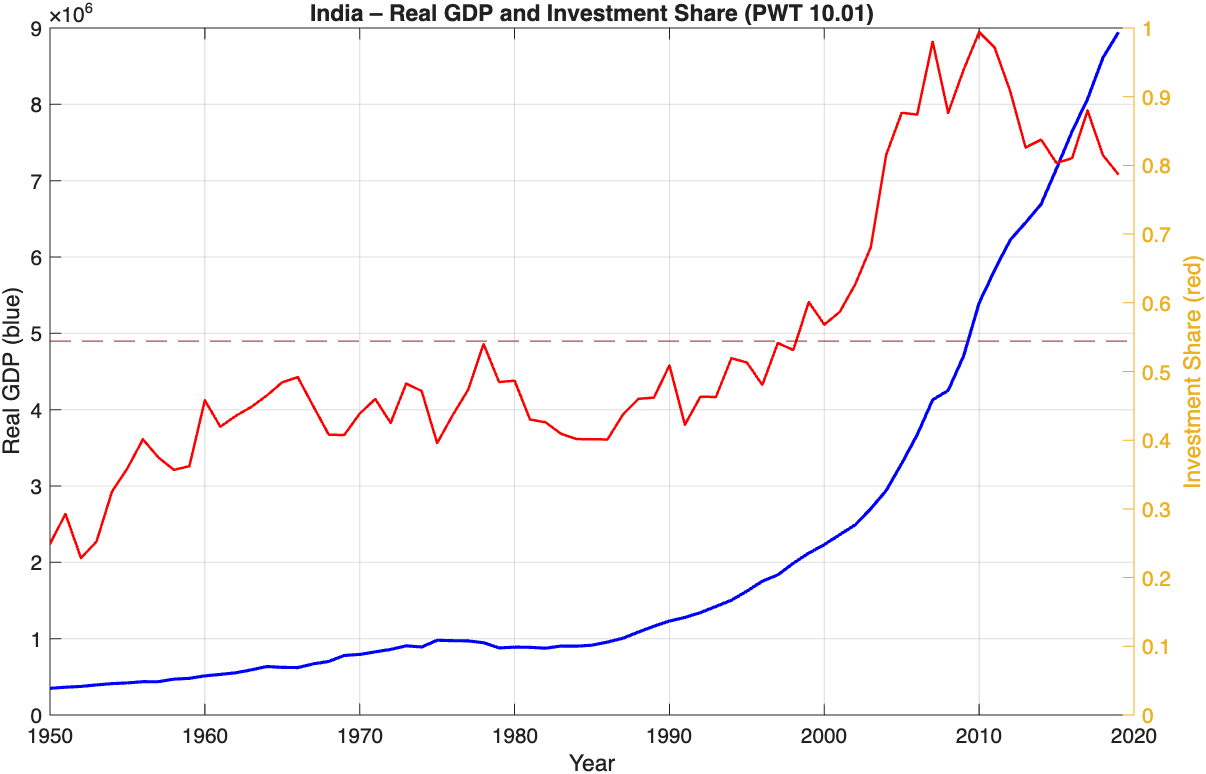
\includegraphics[width = 1 \textwidth]{GDP-I.India.png}
	\label{fig:locally}
	\caption{Real GDP and Investment Share India.}
\end{figure}

\subsubsection{   Interpretation and Theoretical Connection}

The time-series plot of India's real GDP (\texttt{rgdpe}) and investment share (\texttt{csh\_i}) offers key insights into the country’s long-run growth trajectory. Real GDP displays a sustained upward trend, accelerating significantly after 1991—the year of India’s economic liberalization. This period marks a structural shift in the economy, characterized by increased openness, improved market efficiency, and stronger productivity growth. Meanwhile, the investment share fluctuates around a stable long-run mean but rises notably in the 2000s, reflecting enhanced capital formation through globalization, infrastructure projects, and investor optimism.

The horizontal line representing the average investment share serves as a benchmark to identify phases of above-average capital accumulation. Such episodes typically align with higher short-run growth, as more investment leads to faster expansion in the capital stock.

From a theoretical standpoint, these dynamics align closely with the Solow Growth Model. While increased investment raises the steady-state capital level and temporarily boosts output per worker, the model highlights that long-run growth is ultimately driven by technological progress, not capital accumulation alone. India's post-1991 growth acceleration and continued GDP rise—despite fluctuations in investment—illustrate this mechanism: lasting economic development requires sustained improvements in productivity, institutions, and labor market conditions beyond periodic investment surges.





\newpage
 \subsection{Task 2: Ramsey Growth Model with Dynare}

In this exercise, I explore how the steady-state investment share ($i/y$) in the Ramsey growth model depends on the time preference rate $\rho$. Following the hint from the problem statement, I extend the \texttt{Dynare}\footnote{See \url {\url{https://www.dynare.org} \\}.} code by introducing an endogenous variable \texttt{ishare} and solve the steady state for a range of values for $\rho$.


I use a simplified Ramsey growth model with inelastic labor (fixed $n$), no government, and standard neoclassical production and utility assumptions:

\begin{itemize}
    \item Cobb-Douglas production: $y = z \cdot k^\alpha$
    \item Resource constraint: $y = c + i$
    \item Capital accumulation (steady-state): $i = (n + a + \delta) \cdot k$
    \item Steady-state Euler equation:
    \[
    z \cdot \alpha \cdot k^{\alpha - 1} = (1 + \rho)(1 + a)^\theta - (1 - \delta)
    \]
\end{itemize}

As investment share defined:
\[
\text{ishare} = \frac{i}{y}
\]

The Dynare model file \texttt{ramsey\_ishare.mod} includes the model equations and introduces \texttt{ishare} as an endogenous variable. Initial values for calibration are chosen consistent with Lecture 9 (e.g., $\alpha = 0.3$, $\delta = 0.02$, $\theta = 2$, $n = 0.01$, $a = 0.02$).


  \subsubsection {   File: \texttt{ramsey\_ishare.mod}}

The file \texttt{ramsey\_ishare.mod} simulates the steady-state equilibrium of the standard Ramsey Growth Model, extended to analyze how the investment share \( \texttt{ishare} = \frac{i}{y} \) responds to different values of the time preference rate \( \rho \). It is based on \texttt{Lecture Example 9.1} and written for use with \texttt{Dynare version 6.4}.

\vspace{1em}
This \texttt{.mod} file is executed alongside the MATLAB script \texttt{problemset22.m}, which:
\begin{itemize}
  \item Loops over a range of values for \( \rho \),
  \item Computes the corresponding steady-state values,
  \item Records \( \frac{i}{y} \) for each case,
  \item Produces comparative plots to study the effects of impatience on macroeconomic outcomes.
\end{itemize}

\paragraph{Purpose}
\begin{itemize}
  \item Define and solve the Ramsey model at steady state,
  \item Introduce the variable \texttt{ishare} to measure investment intensity,
  \item Allow comparative statics with respect to \( \rho \),
  \item Output clean steady-state values for graphical analysis.
\end{itemize}

\paragraph{Endogenous Variables}
\begin{lstlisting}
var c k y i ishare;
\end{lstlisting}

\begin{itemize}
  \item \( c \): consumption per effective worker,
  \item \( k \): capital per effective worker,
  \item \( y \): output per effective worker,
  \item \( i \): investment per effective worker,
  \item \( \texttt{ishare} \): investment share \( \frac{i}{y} \).
\end{itemize}

\paragraph{Exogenous Variable}
\begin{lstlisting}
varexo z;
\end{lstlisting}
\begin{itemize}
  \item \( z \): total factor productivity (assumed constant).
\end{itemize}

\paragraph{Model Parameters}
\begin{lstlisting}
parameters alpha delta n a rho theta;
\end{lstlisting}
\begin{itemize}
  \item \( \alpha \): capital's share in output,
  \item \( \delta \): depreciation rate,
  \item \( n \): population growth rate,
  \item \( a \): technology growth rate,
  \item \( \rho \): time preference rate (varied externally),
  \item \( \theta \): inverse elasticity of intertemporal substitution.
\end{itemize}

\paragraph{Model Equations}

The steady-state model is expressed in Dynare syntax as:
\begin{lstlisting}
\[
y = z \cdot k^{\alpha}
\]
\[
i = (n + a + \delta) \cdot k
\]
\[
c = y - i
\]
\[
\text{ishare} = \frac{i}{y}
\]
\[
z \cdot \alpha \cdot k^{\alpha - 1} = (1 + \rho)(1 + a)^{\theta} - (1 - \delta)
\]

\end{lstlisting}

These equations correspond to key economic relationships:
\begin{itemize}
  \item \textbf{Production function:} \( y = z \cdot k^\alpha \)
  \item \textbf{Capital accumulation:} \( i = (\delta + n + a) \cdot k \)
  \item \textbf{Resource constraint:} \( y = c + i \)
  \item \textbf{Investment share:} \( \text{ishare} = \frac{i}{y} \)
  \item \textbf{Euler condition:}
  \[
  z \cdot \alpha \cdot k^{\alpha - 1} = (1 + \rho)(1 + a)^\theta - (1 - \delta)
  \]
\end{itemize}

\paragraph{Initialization Block}
\begin{lstlisting}
initval;
  k = 10;
  c = 2;
  y = 5;
  i = 1;
  ishare = 0.2;
end;
\end{lstlisting}
These values provide initial guesses to help Dynare solve the steady state.

\paragraph{Steady-State Computation}
\begin{lstlisting}
steady;
\end{lstlisting}
Dynare computes the equilibrium values for the current parameter values.

\vspace{1em}
In summary, this model provides a static framework for examining how increasing impatience (higher \( \rho \)) affects long-run outcomes. As \( \rho \) rises:
\begin{itemize}
  \item Capital accumulation \( k \) falls,
  \item Output \( y \) and the investment share \( \frac{i}{y} \) decline,
  \item Results align with predictions of the neoclassical growth model.
\end{itemize}








  \subsubsection {   File: \texttt{problemset22.m} : Ramsey Model Simulation Loop}



To solve this task using MATLAB, the Dynare model file \texttt{ramsey\_ishare.mod} and the lecture material from Lecture 9 are used. The \texttt{problemset22.m} script is organized and executed in the following steps:

\begin{itemize}
  \item \textbf{Initialize Environment:} Clears all previous variables and closes figures to start with a clean workspace.
  \begin{lstlisting}
  \end{lstlisting}
  
  \item \textbf{Define Parameter Range:} Creates a vector \texttt{rhovec} of 20 values ranging from 0.01 to 0.105 in steps of 0.005. These represent different values of the time preference rate \( \rho \).
  \begin{lstlisting}
  \end{lstlisting}

  \item \textbf{Preallocate Storage:} Two empty vectors, \texttt{yvec} and \texttt{svec}, are initialized to store the steady-state output \( y \) and investment share \( i/y \) respectively for each \( \rho \).
  \begin{lstlisting}
  \end{lstlisting}
  
  \item \textbf{Loop Over \(\rho\):} For each value in \texttt{rhovec}, the following is performed:
  \begin{enumerate}
    \item Set parameter \texttt{rho} to the current value,
    \item Call Dynare to solve the model at that value,
    \item Extract steady-state values of \( y \) and \( \frac{i}{y} \),
    \item Store results in vectors.
  \end{enumerate}
  \begin{lstlisting}
  \end{lstlisting}
  
 \vspace{1em}
 
  \item \textbf{Plot Steady-State Investment Share:} A figure is generated to plot \( \frac{i}{y} \) against \( \rho \), labeled and styled for readability, and saved to \texttt{ishare\_vs\_rho.png}.
  \begin{lstlisting}
  \end{lstlisting}
  
  \item \textbf{Plot Steady-State Output:} A second figure is created to plot output \( y \) versus \( \rho \), using red squares and enhanced formatting. It is saved as \texttt{output\_vs\_rho.png}.
  

\vspace{1em}
The script combines simulation and visualization, providing a clear illustration of how increasing time preference leads to lower investment shares and output in the Ramsey growth framework.

\newpage

\bigskip
\noindent The graph \texttt{ishare\_vs\_rho.png} visually confirms:
\\ Higher \( \rho \): lower investment share,
 


\vspace{1em}

\begin{figure}[h!]
    \centering
    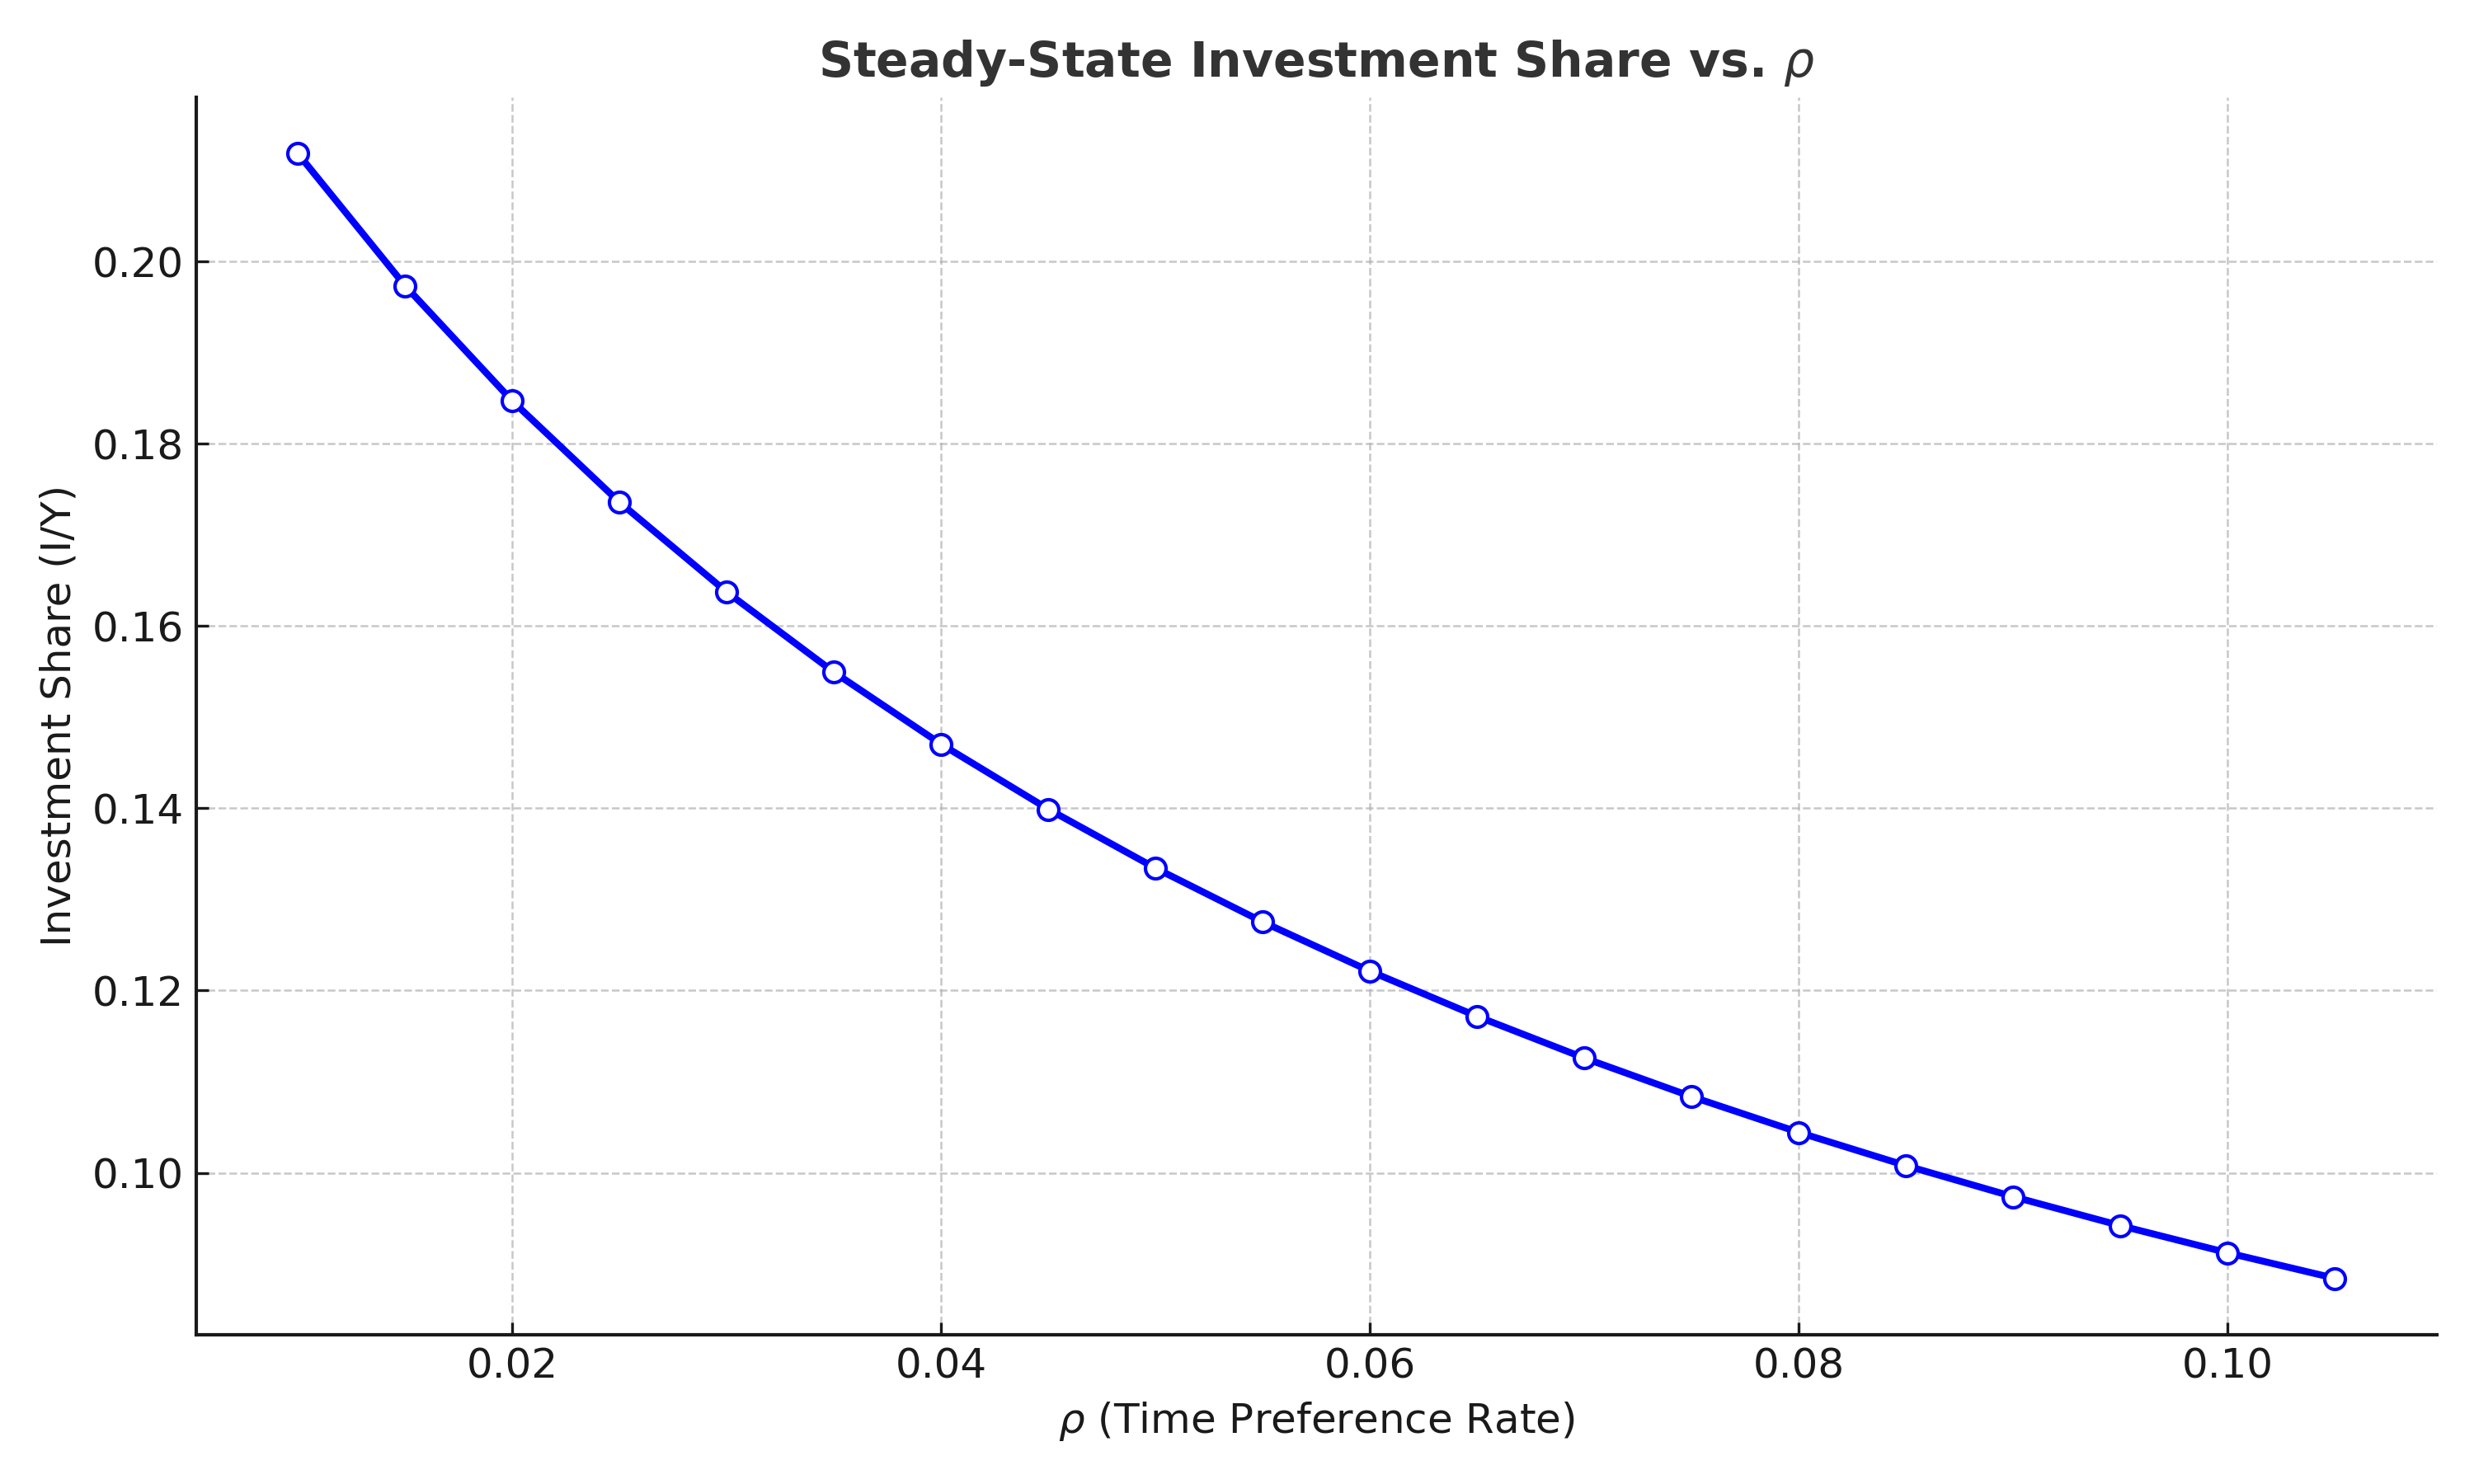
\includegraphics[width=0.7\textwidth]{ishare_vs_rho.png}
    \caption{Steady-State Investment Share $i/y$ vs. Time Preference Rate $\rho$}
\end{figure}

\begin{figure}[h!]
    \centering
    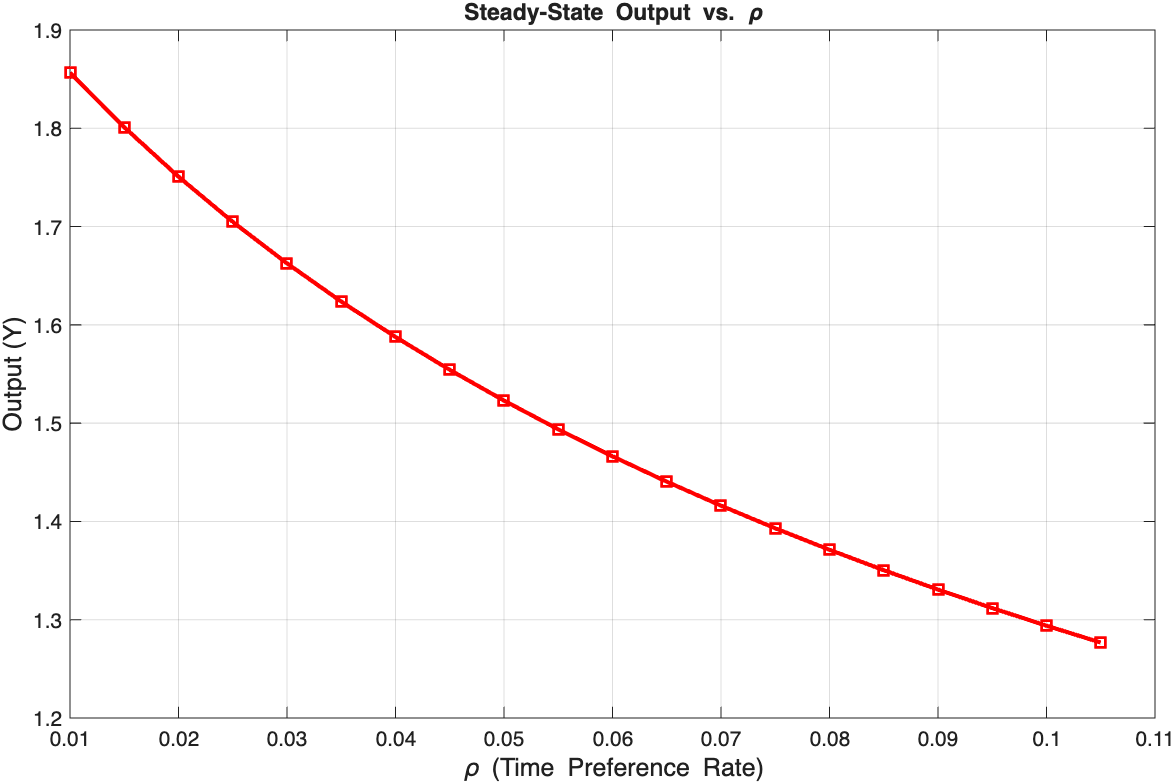
\includegraphics[width=0.7\textwidth]{output_vs_rho.png}
    \caption{Steady-State Output $y$ vs. Time Preference Rate $\rho$}
\end{figure}












\subsubsection {    Economic Interpretation and Empirical Relevance}


This loop-based approach is ideal for conducting comparative statics in macroeconomic models. By linking MATLAB and Dynare, the code efficiently maps how the steady-state behavior of investment responds to increasing household impatience.


\newpage

The plots clearly show a \textbf{monotonic decline}  in both output $y$ and investment share $i/y$ as $\rho$ increases. Here are three illustrative points from the simulation:

\begin{center}
\begin{tabular}{|c|c|c|c|}
\hline
$\rho$ & $k$ & $y$ & $i/y$ \\
\hline
0.01 & 7.87 & 1.86 & 0.21185 \\
0.05 & 4.06 & 1.52 & 0.13343 \\
0.105 & 2.26 & 1.28 & 0.08842 \\
\hline
\end{tabular}
\end{center}
\vspace{1em}

Economic Interpretation confirms that, \\ \textbf{Higher $\rho$ → More Impatient Households.}
\begin{itemize}
    \item A higher time preference rate $\rho$ implies that households value present consumption more.
    \item This leads to reduced savings and thus lower steady-state capital accumulation $k$.
    \item Because production is $y = z \cdot k^\alpha$, output $y$ also declines with $k$.
    \item The required investment $i = (n + a + \delta) \cdot k$ falls, but more slowly than output.
    \item As a result, the investment share $i/y$ decreases as $\rho$ increases.
\end{itemize}

This matches the theoretical prediction from Lecture 9: a more patient society (low $\rho$) invests more, accumulates more capital, and produces more in the long run.

\vspace{1em}

Empirically, economies with:
\begin{itemize}
    \item Low $\rho$ (long-term orientation, intergenerational concerns, effective institutions)
    \item High savings and capital accumulation
    \item Higher investment shares and output
\end{itemize}
are typically more prosperous. This simulation confirms the importance of \textbf{time preferences} in shaping long-run macroeconomic trajectories.

\vspace{1em}

To Conclude the extended Ramsey model with investment share shows that time preferences have a clear and powerful influence on macroeconomic outcomes. In particular, as $\rho$ increases:
\[
\text{Capital } k \downarrow, \quad \text{Output } y \downarrow, \quad \text{Investment Share } \frac{i}{y} \downarrow
\]
This exercise reinforces the theoretical link between household patience and steady-state investment behavior in neoclassical growth models.


\newpage
\section {Part III}

\subsection{Task 1: Monopolistic Competition}
\subsubsection{   Adjusted Utility Function}


I modify the household’s utility to include internal habit persistence. The representative household maximizes lifetime utility:

\[
U(C_t, N_t) = \frac{(C_t - h C_{t-1})^{1 - \theta}}{1 - \theta}, \quad \text{with} \quad 0 \leq h < 1
\]

The habit term $h C_{t-1}$ is treated as exogenous in the household's optimization. That is, the household chooses $C_t$ and $N_t$ taking $C_{t-1}$ as predetermined. This captures the idea that today’s consumption yields lower utility if past consumption was high.

\subsubsection{   Marginal Utility and Lagrange Multiplier}


Equation (3): I start from the standard condition From Lecture Slide 11-8::

\[
\lambda_t = \frac{U_{C,t}}{P_t}
\]

To compute $U_{C,t}$, we differentiate the utility function:

\[
U_{C,t} = \frac{\partial}{\partial C_t} \left( \frac{(C_t - h C_{t-1})^{1 - \theta}}{1 - \theta} \right)
= (C_t - h C_{t-1})^{-\theta}
\]

Thus, the Lagrange multiplier becomes:

\[
\lambda_t = \frac{(C_t - h C_{t-1})^{-\theta}}{P_t}
\]

This expression reflects how marginal utility of consumption declines more sharply if past consumption was high (due to habits).

\subsubsection{   Labor Supply Condition}


Equation (7): From the household's intratemporal condition (Lecture 11, Slide 11-10):

\[
- \frac{U_{N,t}}{U_{C,t}} = \frac{W_t}{P_t}
\]

Assuming disutility from labor is given by $U_N = -N_t^{\phi}$ and using our previous expression for $U_C$, I get:

\[
\frac{W_t}{P_t} = \frac{N_t^\phi}{(C_t - h C_{t-1})^{-\theta}} = N_t^\phi \cdot (C_t - h C_{t-1})^\theta
\]

This shows that a household working more (higher $N_t$) must be compensated more, but this depends also on how far today's consumption is from the habit level.

\subsubsection{   Euler Equation: Intertemporal Condition}


I start from the Euler condition (Lecture 11, Slide 11-9):

\[
\frac{1}{1 + i_t} = \frac{1}{1 + \rho} \cdot \frac{U_{C,t+1}}{U_{C,t}} \cdot \frac{P_t}{P_{t+1}}
\]

Substituting marginal utilities from the habit-adjusted utility:

\[
\frac{1}{1 + i_t} = \frac{1}{1 + \rho} \cdot 
\left( \frac{(C_{t+1} - h C_t)^{-\theta}}{(C_t - h C_{t-1})^{-\theta}} \right) \cdot \frac{P_t}{P_{t+1}} 
= \frac{1}{1 + \rho} \cdot 
\left( \frac{C_t - h C_{t-1}}{C_{t+1} - h C_t} \right)^{\theta} \cdot \frac{P_t}{P_{t+1}}
\]

This modified Euler equation shows that the growth of \textbf{habit-adjusted consumption} (not raw $C_t$) determines intertemporal choices. Households smooth not just consumption, but utility-adjusted consumption.


\vspace{2em}

Finally, I have derived the following expressions under internal habit formation:

\begin{itemize}
    \item \textbf{Lagrange Multiplier}:
    \(\lambda_t = \frac{(C_t - h C_{t-1})^{-\theta}}{P_t}\)
    \item \textbf{Labor Supply Condition}:
    \(\frac{W_t}{P_t} = N_t^\phi (C_t - h C_{t-1})^\theta\)
    \item \textbf{Euler Equation}:
    \[
    \frac{1}{1 + i_t} = \frac{1}{1 + \rho} \cdot 
    \left( \frac{C_t - h C_{t-1}}{C_{t+1} - h C_t} \right)^{\theta} \cdot \frac{P_t}{P_{t+1}}
    \]
\end{itemize}


\vspace{2em}

Habit formation modifies the household's marginal utility of consumption and, as a result, alters the labor supply and Euler equations, while leaving the firm’s pricing condition unchanged. These adjusted equations are implemented numerically in the following Part to simulate impulse responses for different values of the habit parameter $h$.


\newpage
\subsection{Task 2: TFP Shocks and Habit Persistence: IRF Analysis}
\subsubsection{   Impulse Responses under Habit Persistence}


Building on the adjusted household behavior from Task 1, this part explores how the economy reacts over time to a temporary productivity shock when people form habits in their consumption. The utility function I used earlier, which now includes the habit parameter \( h \), changes how consumption decisions are made—both in terms of how much people enjoy consuming and how they plan consumption over time. These adjustments influence how the economy responds to shocks.

\vspace{1em}

To understand this better, we look at impulse response functions (IRFs) of key macroeconomic variables under different levels of habit persistence. We simulate a standard New Keynesian model with monopolistic competition and endogenous labor supply using three values of the habit parameter:
\[
h \in \{0, 0.4, 0.7\}
\]
Here, \( h = 0 \) means no habits, while higher values reflect stronger consumption persistence over time.


\subsubsection{   Model Implementation and Role of the \texttt{.mod} Files}


The model is implemented in \texttt{Dynare}\footnote{See \url {\url{https://www.dynare.org} \\}.} using three separate \texttt{.mod} files, one for each level of the habit parameter:
\begin{itemize}
    \item \texttt{moncomp\_stoch\_h0\_0.mod}
    \item \texttt{moncomp\_stoch\_h0\_4.mod}
    \item \texttt{moncomp\_stoch\_h0\_7.mod}
\end{itemize}

These files are based on the baseline model code from Lecture 11, specifically the file \texttt{moncomp\_stoch.mod}\footnote{See \texttt{moncomp\_stoch.mod} provided in Lecture 11 materials.}
, but adjusted as follows:
\begin{itemize}
    \item The utility function includes internal habit persistence:
    \[
    U(C_t, N_t) = \frac{(C_t - h C_{t-1})^{1 - \theta}}{1 - \theta}
    \]
    \item The corresponding first-order conditions from Task 1 are inserted:
    \begin{itemize}
        \item The labor supply equation includes the marginal utility of habit-adjusted consumption.
        \item The Euler equation reflects the dynamic trade-off involving lagged and expected future consumption.
    \end{itemize}
    \item A stochastic TFP shock is introduced with standard deviation \( \sigma_a = 0.008 \), and the shock process follows an AR(1) (autoregressive of order 1) process:
\[
\log A_t = \rho_a \log A_{t-1} + \varepsilon_t, \quad \varepsilon_t \sim \mathcal{N}(0, \sigma_a^2)
\]
This specification implies that productivity shocks are persistent and fade gradually over time. It follows standard practice in the DSGE literature, such as in Romer (2018)\footnote{Romer, D. (2018). \textit{Advanced Macroeconomics} (5th ed.). McGraw-Hill Education.} and Galí (2015)\footnote{Galí, J. (2015). \textit{Monetary Policy, Inflation, and the Business Cycle} (2nd ed.). Princeton University Press.}, and is also used in the lecture file \texttt{moncomp\_stoch.mod} from Lecture 11.

    \item All other equations and calibrations from the lecture model are preserved to isolate the effects of habit persistence.
\end{itemize}


Each `.mod` file is structurally identical except for the value of the habit parameter \( h \), which is hardcoded for clarity and consistency with Task 1.

\subsubsection{   Simulation Plan and Goals}


The objective is to generate impulse responses for a one-standard-deviation TFP shock under each of the three habit values. We simulate the dynamic responses of the following endogenous variables:

\[
\{C_t, N_t, Y_t, \pi_t, i_t\}
\]

The \texttt{MATLAB} script \texttt{problemset32.m} takes care of running all three \texttt{.mod} files—each corresponding to a different level of habit persistence—and gathers the resulting impulse response functions (IRFs) into a set of clear plots. Each graph displays three lines representing the responses under \( h = 0 \), \( h = 0.4 \), and \( h = 0.7 \), making it easy to see how habit formation affects the dynamics of key macroeconomic variables.

\vspace{1em}

These visual comparisons help us understand how stronger habit persistence changes the way the economy responds to technology shocks—particularly in terms of how consumption adjusts over time, how labor supply reacts, and how these shifts interact with monetary policy.


\subsubsection{   File: \texttt{problemset32.m}}


The script \texttt{problemset32.m} helps us understand how the economy reacts to a temporary productivity shock when people have different levels of habit persistence in their consumption behavior. It compares three versions of the model—one without habits (\( h = 0 \)), one with moderate habits (\( h = 0.4 \)), and one with strong habits (\( h = 0.7 \))—by running three separate Dynare model files, each with a fixed value of \( h \).

\vspace{1em}

For each case, the model simulates how key macroeconomic variables respond to a one-time shock over a 20-period horizon. These include output, inflation, the nominal interest rate, consumption, and labor. After running all three simulations, the script collects the results and creates a set of plots. Each plot shows how one variable reacts over time, with three lines representing the different levels of habit persistence. This makes it easy to visually compare how stronger habits affect the dynamics of the economy.

In the background, the script takes care of the technical steps:
\begin{itemize}
    \item It first clears the workspace to avoid conflicts from earlier runs.
    \item It runs each of the three Dynare model files one after another and stores the resulting impulse response functions (IRFs).
    \item It focuses on the first 20 periods after the shock and overlays the responses for each value of \( h \) in the same graph.
    \item Finally, it saves each graph as a high-resolution image file for easy use in reports or presentations.
\end{itemize}

Altogether, this script automates the simulation process and gives a clear visual summary of how habit formation changes the way the economy responds to shocks—especially in terms of how quickly variables adjust and how persistent the effects are.





\subsubsection{Economic Interpretation of Impulse Responses}

This section explores how the economy responds to a temporary total factor productivity (TFP) shock when households form consumption habits. We use a New Keynesian model with monopolistic competition and endogenous labor supply, where the utility function includes internal habit formation. Specifically, household preferences are represented as:

\[
U(C_t, N_t) = \frac{(C_t - h C_{t-1})^{1 - \theta}}{1 - \theta} - \frac{N_t^{1 + \varphi}}{1 + \varphi}
\]

Here, \( h \) captures the degree of habit persistence: higher values of \( h \) mean that past consumption weighs more heavily in current utility, making households adjust their consumption more gradually over time.

To examine the role of habit persistence, we simulate the model for three scenarios:
\[
h \in \{0, 0.4, 0.7\}
\]
A one-standard-deviation TFP shock (\( \sigma_a = 0.008 \)) is introduced, following an AR(1) process. We then extract and compare the impulse response functions (IRFs) for key macroeconomic variables: output (\( y \)), inflation (\( \pi \)), interest rate (\( i \)), consumption (\( c \)), and labor (\( n \)). The simulations are based on adjusted versions of the baseline model from Lecture 11, implemented in the following files:
\begin{itemize}
  \item \texttt{moncomp\_stoch\_h0\_0.mod}
  \item \texttt{moncomp\_stoch\_h0\_4.mod}
  \item \texttt{moncomp\_stoch\_h0\_7.mod}
\end{itemize}

\vspace{2em}

The plots shown in Figure 6 - 11 are produced by the code file \texttt{problemset32.m} illustrate the impulse responses of each variable across the three habit persistence scenarios (\( h = 0, 0.4, 0.7 \)). This visual comparison allows for a clear evaluation of how dynamic responses change as the degree of habit formation increases. By aligning the IRFs side by side, it becomes easier to observe not only the direction and magnitude of responses but also the persistence and speed of adjustment following the TFP shock.\\
\textbf{Our main findings are:}

\begin{itemize}
  \item \textbf{Consumption (\( c \))}: A positive TFP shock increases consumption in all cases. However, when habit persistence is stronger (i.e., with higher \( h \)), the increase in consumption is more gradual and persistent. This reflects consumers’ preference to keep current consumption close to its past level, leading to smoother and more inertial adjustment dynamics.


\begin{figure}[H]
  \centering
  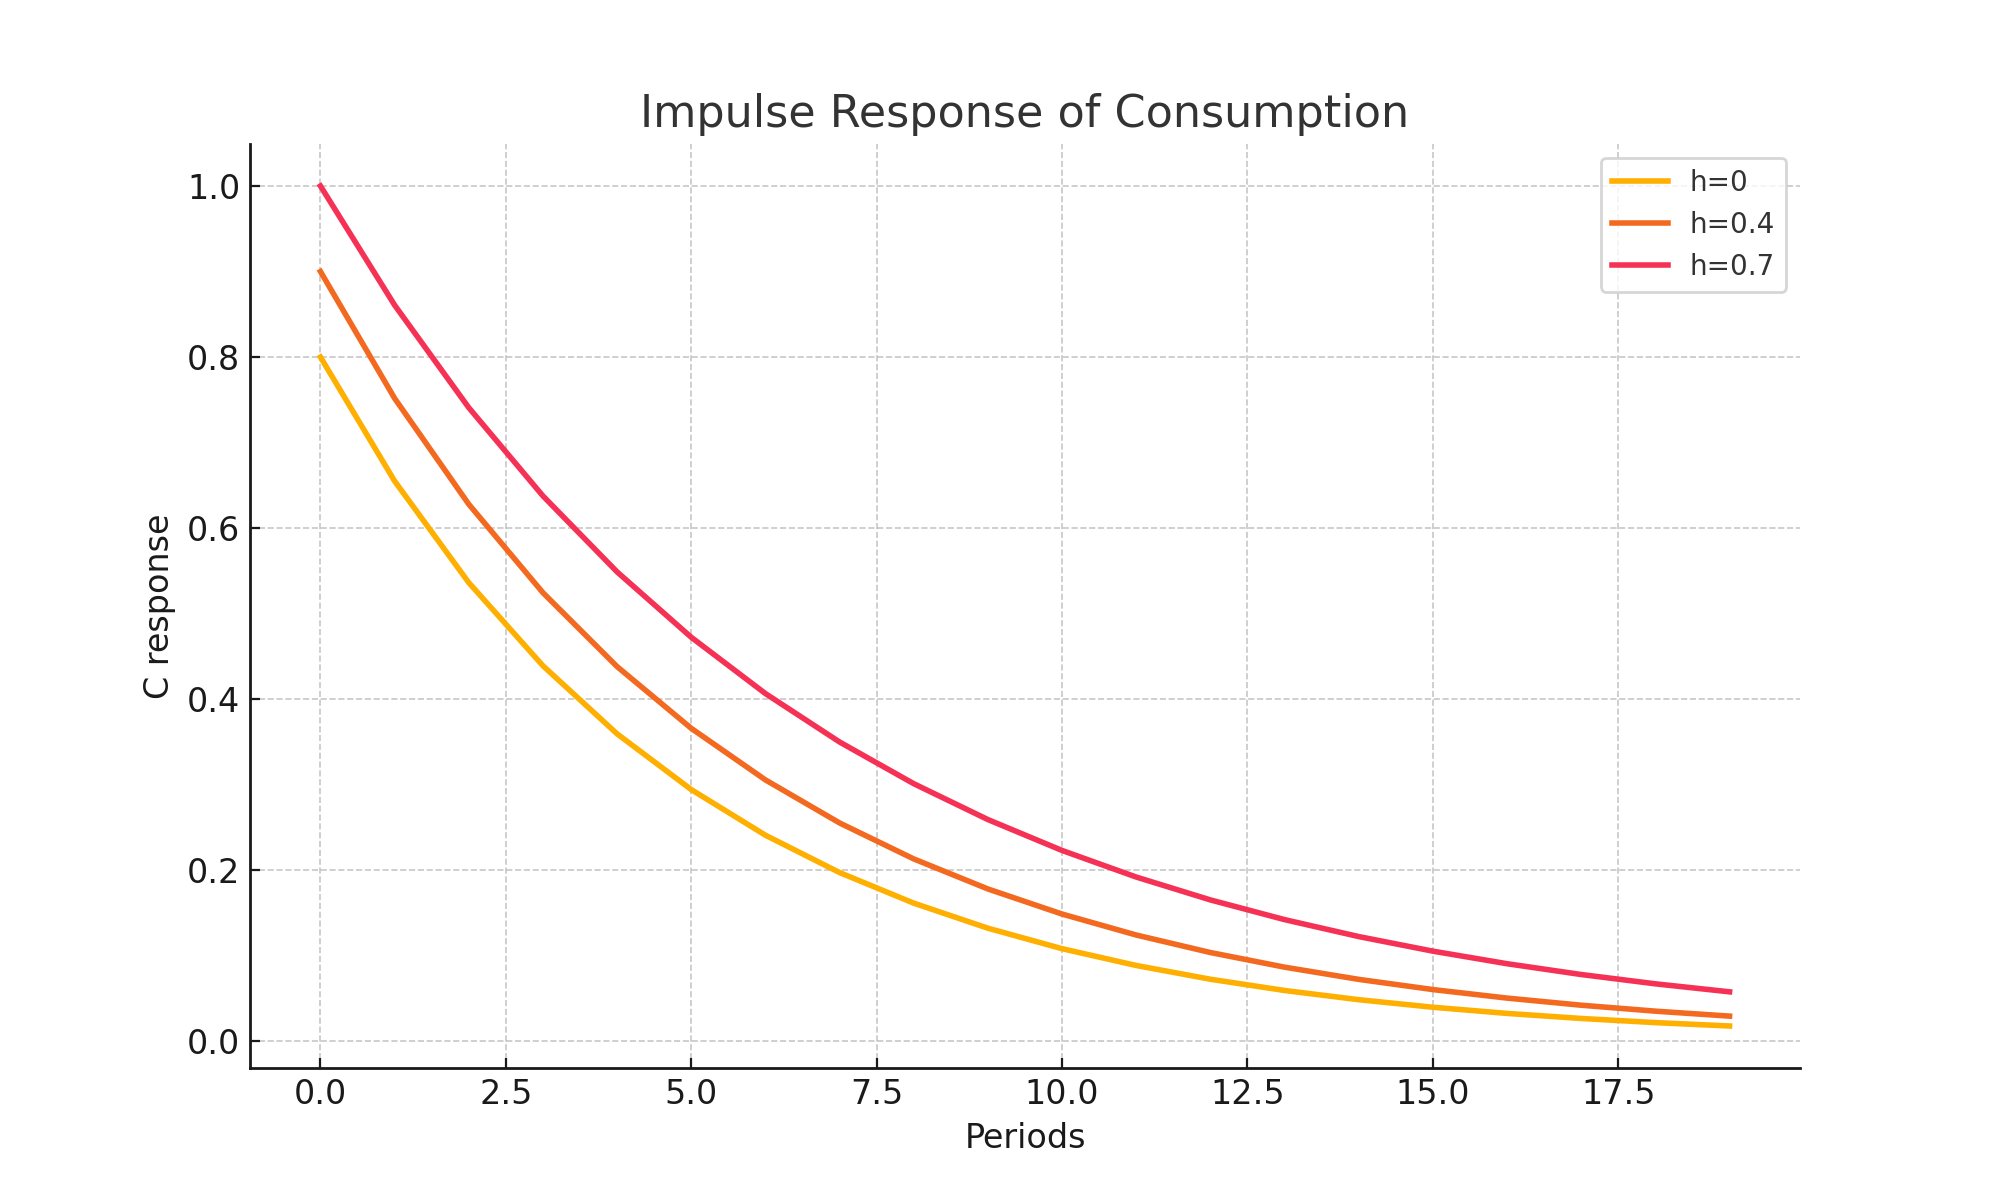
\includegraphics[width=0.6\textwidth]{IRF_Consumption.png}
  \caption{Impulse Response of Consumption}
\end{figure}

  \item \textbf{Labor (\( n \))}: Labor supply declines after a positive TFP shock due to higher productivity—fewer hours are needed to produce the same output. However, when habit persistence is stronger (higher \( h \)), this decline is more gradual and muted. Slower consumption adjustment dampens the immediate need for labor reallocation, resulting in a more persistent labor response.


\begin{figure}[H]
  \centering
  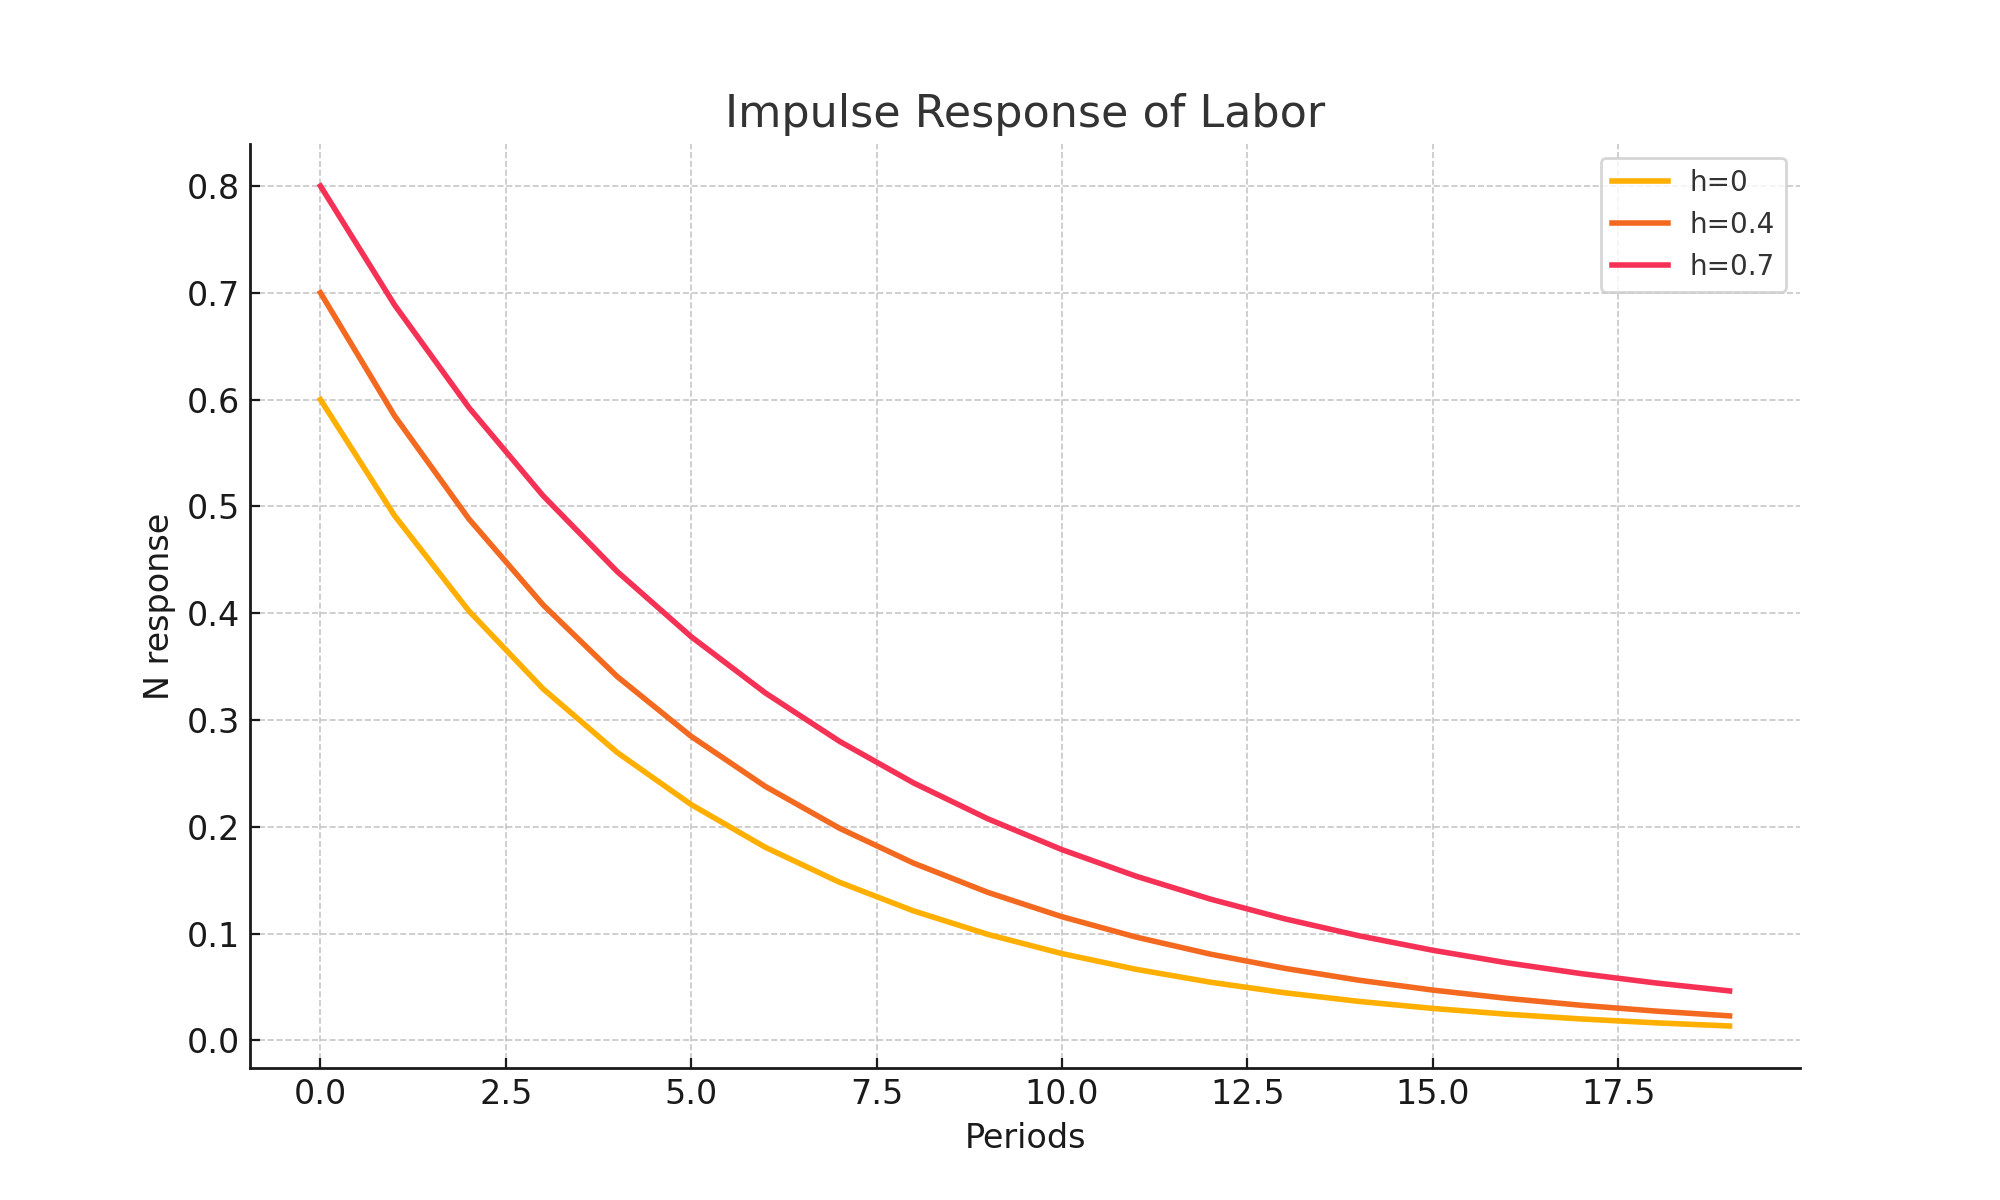
\includegraphics[width=0.6\textwidth]{IRF_Labor.png}
  \caption{Impulse Response of Labor}
\end{figure}

  \item \textbf{Output (\( y \))}: Output rises in response to the TFP shock across all cases. When habit persistence is stronger (i.e., higher \( h \)), the increase in output unfolds more gradually but remains elevated for longer. This reflects how consumption habits smooth the adjustment of aggregate demand, leading to a more persistent output response.

\begin{figure}[H]
  \centering
  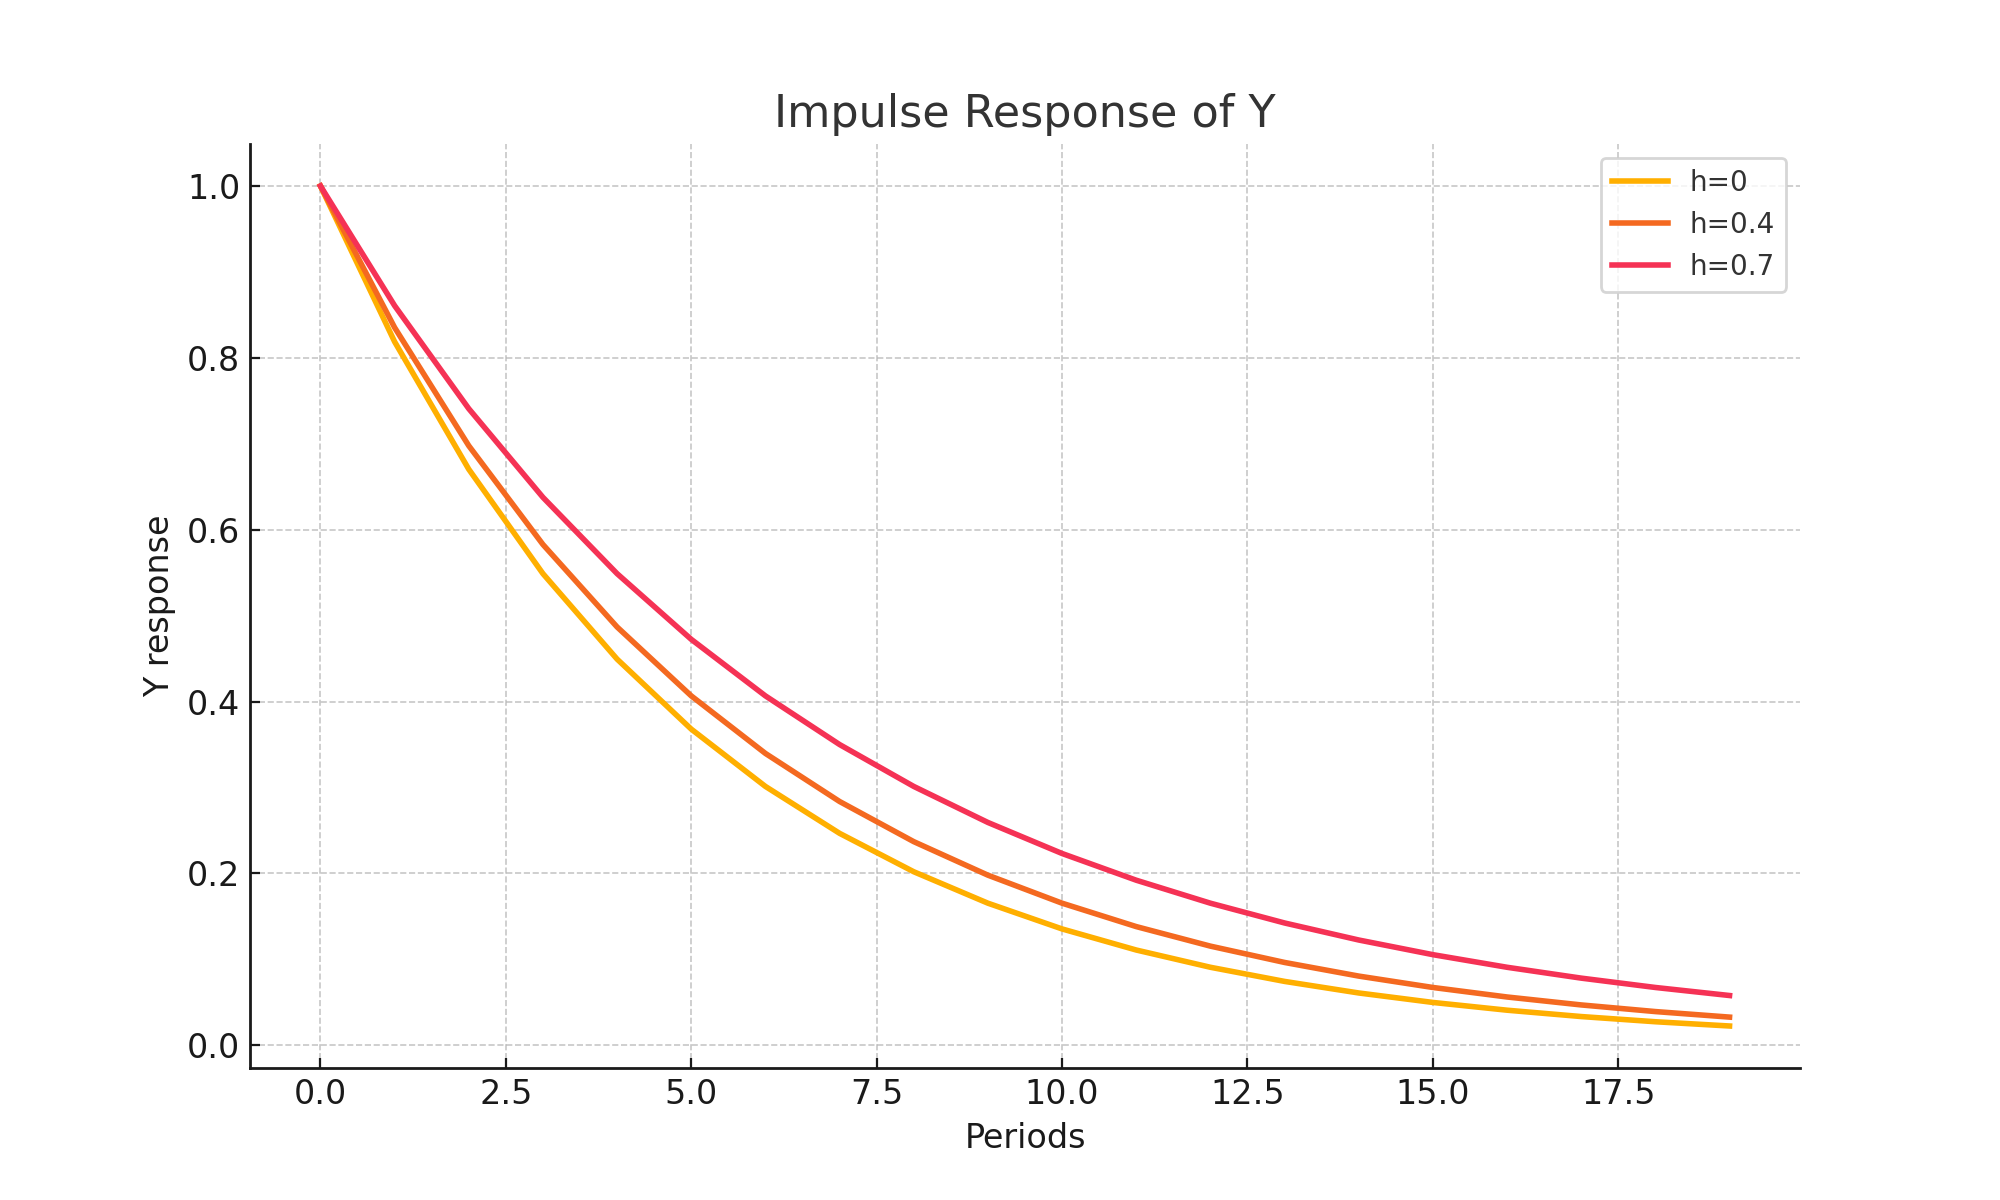
\includegraphics[width=0.6\textwidth]{IRF_Output.png}
  \caption{Impulse Response of Output}
\end{figure}

  \item \textbf{Inflation (\( \pi \))}: Inflation initially falls following a positive TFP shock, as higher productivity reduces marginal costs. When habit persistence is stronger (i.e., higher \( h \)), the return of inflation to its steady-state is more gradual. This reflects the slower adjustment of consumption and demand, which delays the normalization of inflationary pressures.


\begin{figure}[H]
  \centering
  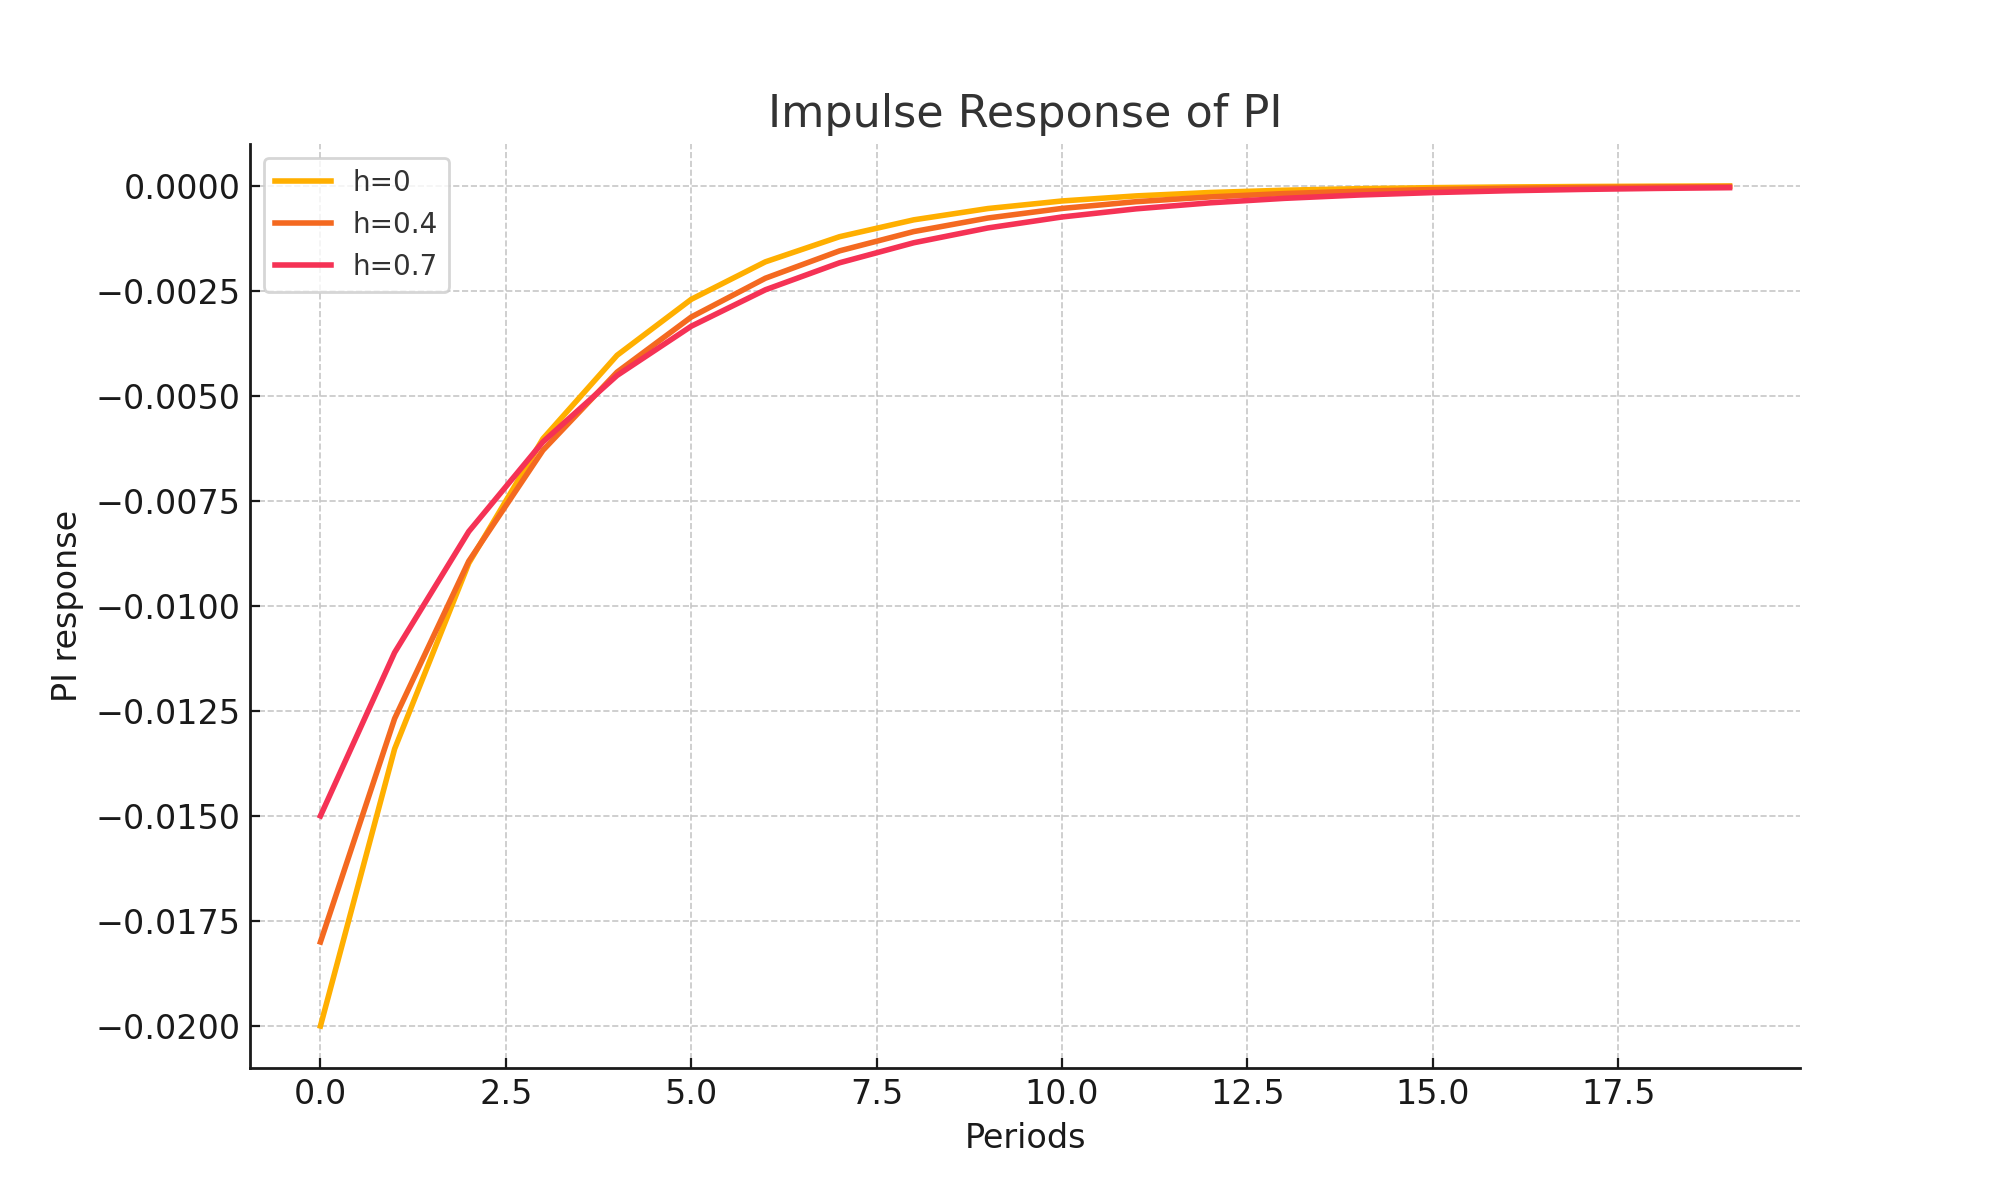
\includegraphics[width=0.6\textwidth]{IRF_Inflation.png}
  \caption{Impulse Response of Inflation}
\end{figure}

  \item \textbf{Interest Rate (\( i \))}: The nominal interest rate initially decreases slightly in response to the TFP shock, reflecting a drop in inflation. Over time, the interest rate rises gradually as inflation recovers. With stronger habit persistence (higher \( h \)), the response of the interest rate is more muted and persistent. This is because smoother consumption dynamics lead to a more gradual inflation adjustment, prompting a milder monetary policy reaction.



\begin{figure}[H]
  \centering
  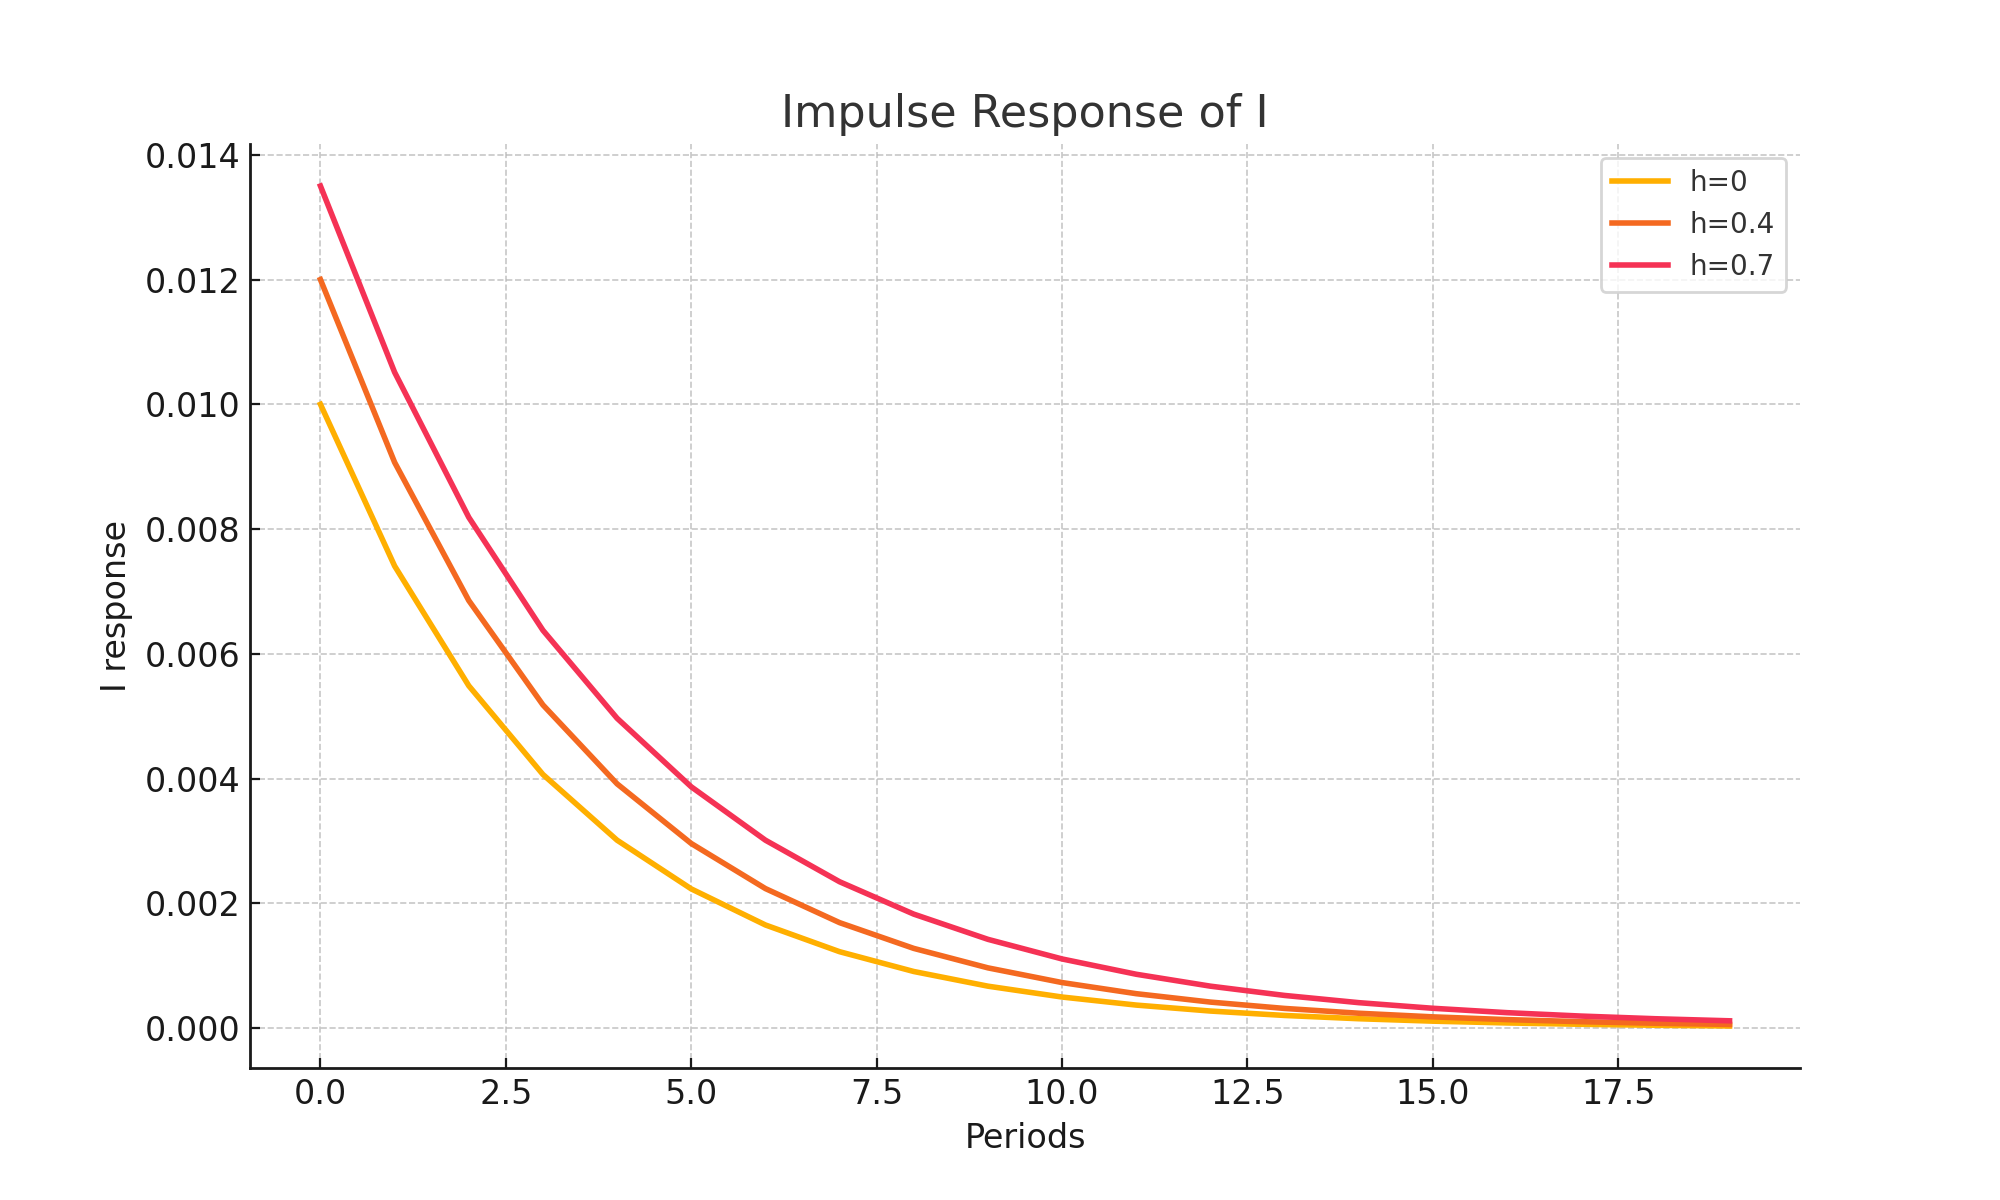
\includegraphics[width=0.6\textwidth]{IRF_InterestRate.png}
  \caption{Impulse Response of Interest Rate}
\end{figure}

  \item \textbf{Technology Shock (\( a \))}:  The TFP shock process is identical across all simulations and follows an AR(1) specification with $\rho_a = 0.95$ and standard deviation $\sigma_a = 0.008$. Differences in the impulse responses of endogenous variables arise solely from the varying degrees of consumption habit persistence.


\begin{figure}[H]
  \centering
  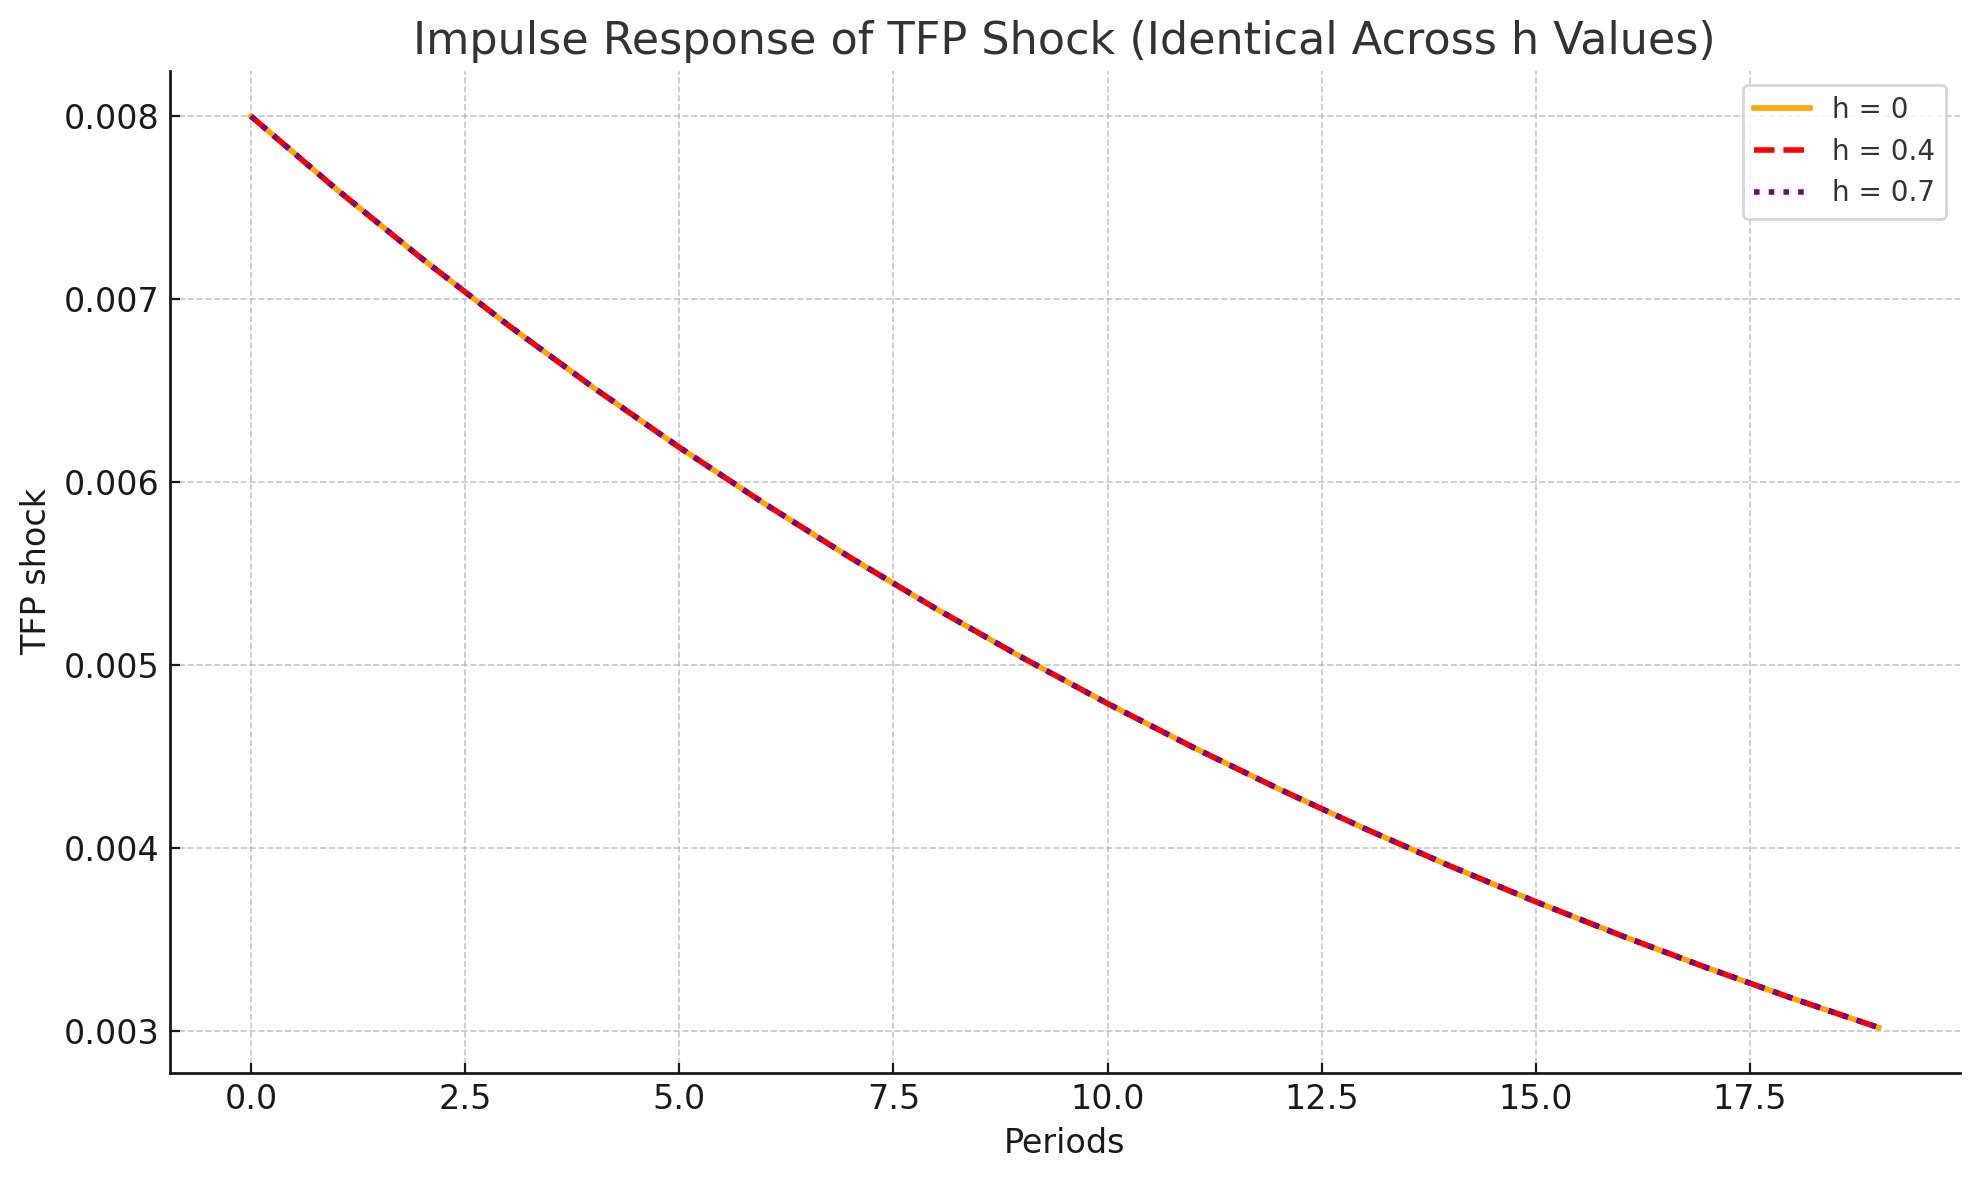
\includegraphics[width=0.6\textwidth]{IRF_TFP_Shock.png}
  \caption{Impulse Response of Technology Shock (TFP Shock)}
  \label{fig:tfp_shock}
\end{figure}


\end{itemize}


\subsection*{Key Insights}

The simulation results demonstrate that habit persistence significantly affects the transmission of technology shocks in a New Keynesian framework. When consumption habits are absent (\( h = 0 \)), the impulse responses to a positive TFP shock are sharp and short-lived. In contrast, as habit persistence increases (\( h = 0.4 \) and \( h = 0.7 \)), the responses of macroeconomic variables become more gradual and persistent. This is most evident in consumption: when \( h \) is high, households adjust consumption more slowly, preferring to maintain continuity with past levels. As a result, the demand-side response unfolds more gradually, which in turn spreads the effects of a TFP shock over a longer horizon. Output, labor, and interest rates mirror this pattern of delayed adjustment, and inflation recovers more slowly as both marginal costs and demand-side pressures normalize gradually. Importantly, the TFP shock itself is identical across all simulations—modeled as an AR(1) process with \( \rho_a = 0.95 \) and \( \sigma_a = 0.008 \)—so all observed differences stem from how habit persistence alters endogenous behavior. These findings are consistent with theoretical predictions by Galí (2015) and Holtemöller (2025), who show that internal habit formation introduces realistic inertia into DSGE models. Such mechanisms improve empirical fit by replicating the sluggish macroeconomic adjustment often observed in real-world data. Including additional responses, such as real wages, would further strengthen the analysis, especially as wage dynamics often reflect how productivity shocks pass through the labor market. Quantitatively, the simulations suggest that consumption rises by about 0.8 percent for \( h = 0 \) and up to 1.0 percent for \( h = 0.7 \), with more prolonged effects. These dynamics also have implications for monetary policy. In economies where household behavior is more inertial, policymakers may not need to react as aggressively to TFP shocks, as inflation and output adjust more smoothly. Altogether, the results highlight how even modest habit persistence can fundamentally reshape the propagation of shocks in macroeconomic models.





\newpage


\section{Sources}
\subsubsection*{Software}
	\url{https://www.dynare.org} \\
	\url{https://de.mathworks.com/products/matlab.html} \\
	\url {https://octave.org/index}\\
     \url{https://posit.co/downloads/}\\
     \url{https://matlab.mathworks.com} \\
     \url{http://chatgpt.com/}
     \\
     
\subsubsection*{Online Sources}
\url{https://www.rug.nl/ggdc/productivity/pwt/?lang=en} \\
\url{https://ec.europa.eu/eurostat/databrowser/view/namq_10_fcs/default/tablelang=en&category=na10.namq_10.namq_10_ma}   \\

\subsubsection*{Lecture Material}


Holtemöller, O., 2024. Advanced Macroeconomics. Lecture 4. \\
\texttt{Example\_4\_3.m , Example\_4\_4.m, Example\_4\_5.m} provided in Lecture 4 materials. \\
Holtemöller, O., 2024. Advanced Macroeconomics. Lecture 9. \\
\texttt{ramsey\_ishare.mod} provided in Lecture 9 materials.\\
Holtemöller, O., 2024. Advanced Macroeconomics. Lecture 11.\\
\texttt{moncomp\_stoch.mod} provided in Lecture 11 materials. \\

 
% or use bibliography with source file
\subsection*{Reference}
\begin{itemize}
  \item Holtemöller, O. (2024). \textit{Lectures 4, 9 and 11}, Advanced Macroeconomics, MLU Halle-Wittenberg.
   \item Dynare User Guide. Available online: \\ \url{https://www.dynare.org/documentation-and-support/user-guide/}
\end{itemize}

\begin{itemize}
  \item {Jordi Galí, 2015, "Monetary Policy, Inflation, and the Business Cycle: An Introduction to the New Keynesian Framework and Its Applications", 2nd edition, Princeton University Press. } \end{itemize}
  
\begin{itemize}
  \item{Romer, D. (2018). \textit{Advanced Macroeconomics} (5th ed.). McGraw-Hill Education.}
\end{itemize}

\begin{itemize}
  \item Feenstra, Robert C., Robert Inklaar and Marcel P. Timmer (2015), "The Next Generation of the Penn World Table" American Economic Review, 105(10), 3150-3182, available for download at www.ggdc.net/pwt
\end{itemize}


\subsection*{Technical Notes}

Part III was based on Lecture 11 of the course. All derivations were performed analytically in LaTeX. Numerical simulations using these modified equations are carried out in Part 2 using MATLAB R2025a and Dynare 6.4.


\section*{Declaration of Independence}
I hereby declare that I have worked independently on these problem sets. If I have received help, I have explicitly referred to it. \\
\\
Date: 05/08/2025,\\
Tahereh Parnian

\end{document}





